\documentclass[]{article}

\usepackage[utf8]{inputenc}
\usepackage[T1]{fontenc}
\usepackage[english]{babel}

\usepackage[pdftex]{graphicx}
\usepackage{latexsym}
\usepackage{tikz}
\usepackage{forest}
\usepackage{subcaption}
\usepackage{amsmath,amssymb,amsthm}
\usepackage{mathtools}
\usepackage{algorithm}
\usepackage[titletoc]{appendix}
\usepackage[noend]{algpseudocode}
\usepackage{listings}
\usepackage{float}
\usepackage{caption}
\usepackage{array}
\usepackage{enumitem}

\usetikzlibrary{arrows,automata,trees,graphs}
\newcommand{\pushcode}[1][1]{\hskip\dimexpr#1\algorithmicindent\relax}
\setlength{\topmargin}{-15mm}
\setlength\extrarowheight{2pt}

\lstset{basicstyle=\footnotesize, tabsize=4, language=Python}

\newtheorem{theorem}{Theorem}[section]
\newtheorem{proposition}[theorem]{Proposition}
\newtheorem{lemma}[theorem]{Lemma}
\newtheorem{definition}[theorem]{Definition}
\newtheorem{corollary}[theorem]{Corollary}
\newtheorem{observation}[theorem]{Observation}
\newtheorem{remark}[theorem]{Remark}
\newtheorem{example}[theorem]{Example}

\numberwithin{equation}{section}

\begin{document}
% Keine Seitenzahlen im Vorspann
\pagestyle{empty}

% Titelblatt
\begin{titlepage}
	
	\vspace*{2cm} 
	
	\begin{center} \large 
		
		Bachelor Thesis
		\vspace*{2cm}
 		
 		{\huge Formal-Language-Constrained Path Problems}
 		\vspace*{2.5cm}
 		
 		Felix Hoffmann
 		\vspace*{1.5cm}
 		
 		$9^{th}$ of August, 2016
 		\vspace*{4.5cm}
 		
 		
 		Supervisor: Prof. Dr. Sven O. Krumke \\[1cm]
 		Department of Mathematics \\[1cm]
 		TU Kaiserslautern
 		
 	\end{center}
\end{titlepage}

% Inhaltsverzeichnis
\tableofcontents

\newpage

% Ab sofort Seitenzahlen in der Kopfzeile anzeigen
\pagestyle{headings}

\section{Introduction}
\label{sec:intro}

Graphs and networks are powerful modeling tools in scientific, engineering, economic and mathematic problem areas. Developing and analyzing efficient methods for solving problems on graphs is a major step towards finding solutions to many practical problems. Thus, the shortest path problem is one of the most basic and best-studied problems in combinatorial optimization.\\

However, in many path-finding problems the desired path is not necessarily the shortest path. Often edges are labeled and only paths with certain patterns of edge labels are candidates for the wanted path, while others are not interesting. Thus, the feasibility of a path is determined by its cost and its labels. The allowed label patterns can be modeled as a formal language. Concatenating the labels of the edges on a shortest path must then form a word of the language. For example, consider a road network where roads are differentiated by categories (highways, local streets, railroad tracks etc.). A traveler can choose different mode options to reach his destination. A formal language specifies the mode selection and destination patterns of possible routes. Another example is the $k$-similar-path problem, where two shortest paths between the same pair of vertices are computed. Thereby, the second path is not allowed to reuse more than $k$ edges of the first one. This is useful, for instance, to avoid traffic jams in vehicle routing. For a third, somewhat simpler example of mode restrictions consider a pedestrian bridge. Since cars are not able to use this bridge we need to prevent routing them across it. Similarly, highways should not be used as parts of routes for pedestrians or cyclists. Updating the road network for every single routing question is costly and needs to be prevented. Instead, we label the graph with information needed to deal with these problems.\\

The purpose of this thesis is to generalize, study and solve the point-to-point single-source shortest path problem with the additional constraint that the label of the path has to belong to some formal language. We mainly use, show and refer to the results of \cite{BJM00} and extend those for special cases. Our goal is to give an idea of the practical consequences of solving shortest path problems with formal language constraints. Specific contributions discussed in this thesis include the following:

\begin{enumerate}
	\item We take a look at solving shortest path problems efficiently on unlabeled graphs. Thereby, certain graph classes (namely, directed acyclic and series-parallel graphs) are considered.
	
	\item We describe a generalization of Dijkstra’s algorithm to finding shortest paths that obey regular language constraints and how to efficiently implement it. Also, some speed-up techniques are stated.
	
	\item Next, we show a polynomial-time algorithm for context-free-constrained shortest paths.
	
	\item We investigate language-constrained simple path problems, their hardness and present an algorithm for solving them on treewidth-bounded graphs.
	
	\item We study the efficiency of our algorithms in terms of running time.
\end{enumerate}

\subsection{Related Work}
\label{sec:intro:rel}

We refer the reader to \cite{KN12} by Krumke and Noltemeier and to \cite{Die06} by Diestel for a comprehensive introduction to graph theory and path problems. The books \cite{HMU06} by Hopcroft, Motwani and Ullmann and \cite{Sch08} by Sch\"oning are a broad survey on automata theory and languages. Furthermore, formal language constrained path problems were previously discussed in great detail in various papers, including \cite{BJM00} by Barret, Jacob and Marathe and \cite{BB+08} by Barret, Bisset, Holzer, Konjevod, Marathe and Wagner. This thesis is greatly based upon these works.\\

We present the algorithms for regular and context-free language-constrained shortest path problems proposed by \cite{BJM00} and \cite{WWB08} in section \ref{sec:shp}. The algorithm for the context-free language-constrained simple path problem by \cite{BJM00} is shown in section \ref{sec:sip}. The remainder of the thesis is organized as follows. Section \ref{sec:found} defines the formal-language-constrained shortest path problem and refers to some applications. Basic definitions are given in section \ref{sec:def}. In section \ref{sec:unlabeled}, we present efficient linear time algorithms for unlabeled shortest path problems on special graph classes (namely, directed acyclic and series-parallel graphs). Starting with section \ref{sec:study} we investigate running times of our implementations on graphs and networks of different sizes. Section \ref{sec:ext} states some extensions to the problem which could be of interest for further discussion and section \ref{sec:conclusion} lists our results.\\

Our initial motivation for studying shortest paths came from a group project at our university and built the basis of this thesis.

\newpage

\section{Foundation}
\label{sec:found}

In this section, we define the formal-language-constrained shortest-path problems.

\subsection{Problem Statement}
\label{sec:found:problem}

The problems discussed here can be formally described as follows: Let $G=(V,E)$ be a directed graph. A \textit{source} of a graph is a vertex with in-degree zero, a \textit{sink} is a vertex with out-degree zero. We indicate the \textit{weight} or \textit{cost} of an edge $e \in E$ with $w(e)$ and assume that these are nonnegative integers. Furthermore $l(e)$ denotes the \textit{label} of $e$ and is an element of a finite alphabet $\Sigma$.\\

A \textit{path} $p$ of length $k$ from $s$ to $t$ in $G$ is a sequence of edges $e_1, e_2, ...,e_k$ such that $e_1 = (s, v_1), e_k = (v_{k-1},t)$, and $e_i = (v_{i-1}, v_i)$ for $1 < i < k$. The \textit{weight} of the path $p = e_1, e_2, ..., e_k$ is given by $\sum_{i=1}^{k} w(e_i)$ and the \textit{label} of $p$ is defined as $l(e_1) \cdot l(e_2) \cdot \cdot \cdot l(e_k)$ concatenating the labels of the edges on the path. Let $w(p)$ and $l(p)$ denote the weight and the label of $p$, respectively.\\

Following the existing literature on shortest path problems, our paths are allowed to repeat vertices. In fact, our paths are allowed to be $walks$, that is, they may even repeat edges. When neither edge nor vertex repetition is allowed, we use the term $simple$ $path$.

\begin{definition}[formal-language-constrained shortest path problem]
	\label{def:langconshp}
	Given a finite alphabet $\Sigma$, a labeled, weighted graph $G = (V,E)$, a source $s$, a destination $t$ and a formal language $L\subseteq \Sigma^*$, find a shortest (not necessary simple) $s$-$t$-path $p$ in $G$ such that $l(p) \in L$.
\end{definition}

\begin{definition}[formal-language-constrained simple path problem]
	\label{def:langconsip}
	Given a finite alphabet $\Sigma$, a labeled, weighted graph $G = (V,E)$, a source $s$, a destination $t$ and a formal language $L\subseteq \Sigma^*$, find a shortest simple $s$-$t$-path $p$ in $G$ such that $l(p) \in L$.
\end{definition}

Note that a shortest path between $s$ and $t$ in unlabeled graphs with edge weights strictly greater than zero, is necessarily simple. This is not the case when we want to find a shortest path satisfying some additional formal language constraints. As an example, consider the graph $G=(V,E)$ (cf. figure \ref{fig:spnotsimple}) that is a four node cycle. Let all edges have weight 1 and label $a$. Now look at two adjacent vertices $v_1$ and $v_2$. The shortest path from $v_1$ to $v_2$ is just a single edge between them, but a shortest path with label $aaaaa$ consists of a whole cycle starting at $v_1$ and the additional edge $(v_1, v_2)$.\\

\begin{figure}[H]
	\centering
	\begin{tikzpicture}
	[scale=.6,auto=middle]
	\node[circle, draw] (n1) at (0,2) {$v_1$};
	\node[circle, draw] (n2) at (2,4)  {$v_2$};
	\node[circle, draw] (n3) at (4,2)  {$v_3$};
	\node[circle, draw] (n4) at (2,0) {$v_4$};
	
	\foreach \from/\to in {n1/n2,n2/n3,n3/n4,n4/n1}
	\draw (\from) -- (\to) node[midway,sloped,above] {$a$};
	\end{tikzpicture}
	\caption{Label constrained shortest paths are not necessary simple}
	\label{fig:spnotsimple}
\end{figure}

For the rest of this thesis, the formal-language-constrained shortest path problem restricted to regular and context-free languages are abbreviated with REG-ShP and CFG-ShP. Analogously we denote the formal-language-constrained simple path problem restricted to regular and context-free languages with REG-SiP and CFG-SiP.\\

In general, the input for these problems is assumed to consist of a description of the graph (with labels and weights) together with the description of the formal language. The problem can be modified by restricting the graph and/or the language.

\subsection{Applications}
\label{sec:found:app}
We provide some examples to illustrate types of problems solvable using the label constrained modeling framework we have discussed.\\

\noindent \textit{Multimodal Networks}. Consider a multimodal network, which is a network with multiple mode choices, such as traveling by vehicles like cars, planes, trains, etc. We wish to find shortest paths satisfying certain mode-choice constraints. Through evaluating real-life survey data the necessary statistical models for obtaining each traveler's mode choice can be built.

\begin{example}
	\label{ex:routing}
	 Suppose we are given a road network in terms of a directed weighted graph $G$. Consider a traveler who wants to take a bus from a start $s$ to a destination point $t$. This is known as the shortest-path problem. But additionally, the traveler either wants to walk from $s$ to a train station and from a train station to $t$ or he drives the whole way with a car. To take those modal choices in account, we add a vertex for each train station and an edge between each consecutive pair of stations to our given network $G$. The edges are labeled according to the allowed travel modes ($c$ for car travel, $w$ for walking on pedestrian paths and $t$ for train tracks). If the network contains a $w$-labeled edge with length zero for each change of train, we can model the traveler’s restriction as $w^*t^*w^*\cup c^*$.
\end{example}

\noindent \textit{k-Similar Paths}. As a second application, we wish to find two shortest paths from $s$ to $t$ for vehicle routing. Thereby the second path is only allowed to use at most $k$ edges passed by the first one. This can be useful, e. g., to plan for a travel group different transfers between two fixed points or to bypass traffic jam on the first route. Depending on the network and the choice of $k$ the length of the second path may be greater than the length of the first path.

\begin{example}
	\label{ex:kpath}
	Given a directed weighted graph $G$ which again represents a transportation network we want to find two paths from $s$ to $t$ with no more than $k$ edges in common. One way to do this is by calculating a shortest $s$-$t$-path $p$ in the given network, labeling $p$’s edges by $t$ (for taken) and all remaining ones by $f$ (for free). Then solving the $s$-$t$-query again for the expression $f^*(t \cup f^*)^kf^*$ yields the desired solution. Another way of solving this problem is by giving all edges used by the first path a resource cost of one and then solving the resource constrained shortest path problem (RCSP) with the condition that at most $k$ resources are used. For more information about RSCP, we refer to \cite{ID05}.
\end{example}

\noindent \textit{Web Searching}. Database searches and browsing the World Wide Web can also be viewed as navigating through certain networks. Imagine the Web as a directed, labeled graph. Each node is a URL site and each edge represents a hyperlink. By following links one can browse the network in search of a particular URL site. This is basically a formal-language-constrained (shortest) path problem where every edge has weight one.

\newpage

\section{Basic Definitions}
\label{sec:def}

We recall the basic concepts in formal language and graph theory.

\subsection{Formal Languages}
\label{sec:def:lang}

\begin{definition}[formal language]
	\label{def:language}
	A formal language $L$ over an alphabet $\Sigma$ is a subset of $\Sigma^*$. An alphabet $\Sigma$ is a finite set of distinguishable symbols or characters. $\Sigma^*$ is the Kleene closure of $\Sigma$, in other words, $\Sigma^*$ is the set of all strings over $\Sigma$.
\end{definition}

\begin{definition}[grammar]
	\label{def:grammar}
	A grammar is formally defined as the tuple $G = (N,\Sigma ,P,S)$, where:
	\begin{itemize}
		\item[(i)] N is a finite set of nonterminal symbols, that is disjoint with the strings formed from G.
		\item[(ii)] $\Sigma$ is a finite set of terminal symbols that is disjoint from N.
		\item[(iii)]  P is a finite set of production rules, each rule of the form $(\Sigma \cup N)^*N(\Sigma \cup N)^*\rightarrow (\Sigma \cup N)^*$.
		\item[(iv)] $S\in N$ is a distinguished symbol that is the start symbol.
	\end{itemize}
	Furthermore, each grammar implicitly defines a language $L(G)\coloneqq \{w\in\Sigma^*:S\Rightarrow^*w\}$. Here $\Rightarrow^*$ means deriving S finitely many times according to the production rules $P$ of the grammar $G$.
\end{definition}

\begin{example}
	\label{ex:langofgrammar}
	Let $G=(N,\Sigma,P,S)$ be a grammar with $N = \{S\}$, $\Sigma = \{a,b\}$ and $P = \{S\rightarrow aSb, S \rightarrow ab\}$.\\
	Deriving the start symbol $S$ directly yields $aSb$; from $aSb$ we can derive $aaSbb$ and using the production $S \rightarrow ab$ on $aaSbb$ we get $aaabbb$.	The sequence $S \rightarrow aSb \rightarrow aaSbb \rightarrow aaabbb$ is the deriving sequence for $aaabbb$.\\
	The language defined by $G$ is 
	$$L(G)=\{a^nb^n:n\in\mathbb{N}\backslash\{0\}\}.$$
\end{example}

\begin{definition}[regular expression]
	\label{def:regex}
	Let $\Sigma$ be a finite alphabet disjoint from $\{\varepsilon, \emptyset, (, ),\bigcup, \cdot, *\}$. A regular expression $R$ over $\Sigma$ is defined as follows:
	\begin{itemize}
		\item[(i)] The empty string "$\varepsilon$", the empty set "$\emptyset$" and, for each	$a \in \Sigma$, "$a$" are atomic regular expressions.
		\item[(ii)] If $R_1$ and $R_2$ are regular expressions, then ($R_1 \cup R_2$), ($R_1 \times R_2$), and $R_1^*$	are compound regular expressions.
	\end{itemize}
\end{definition}

\begin{definition}
	\label{def:langbyregex}
	Given a regular expression $R$, the language (or the set) defined by $R$ over $\Sigma$ and denoted by $L(R)$ is defined as follows:
	\begin{itemize}
		\item[(i)] $L(\varepsilon) = \{\varepsilon\}$, $L(\emptyset) = \emptyset$, $\forall a	\in \Sigma: L(a) = \{a\}$;
		\item[(ii)] $L(R_1 \cup R_2) = L(R_1) \cup L(R_2) = \{w | w \in L(R_1)$ or $w \in L(R_2)\}$;
		\item[(iii)] $L(R_1 \times R_2) = L(R_1) \times L(R_2) = \{w_1w_2 | w_1 \in	L(R_1)$ and $w_2 \in L(R_2)\}$;
		\item[(iv)] $L(R^*) = \bigcup_{k=0}^{\infty} L(R)^k$, where $L(R)^0 = \{\varepsilon\}$	and $L(R)^i = L(R)^{i-1}\times L(R)$.
	\end{itemize}
\end{definition}

\begin{example}
	\label{ex:langbyregex}
	Let $R = (a|ab)^*$ be a regular expression. Then the language defined by $R$ is
	$$L(R) = \{(a|ab)^n:n \in \mathbb{N}\}.$$
\end{example}

\begin{definition}[NFA]
	\label{def:nfa}
	A nondeterministic finite automaton (NFA) is a tuple $M = (S, \Sigma, \delta, s_0, F)$, where
	\begin{itemize}
		\item[(i)] $S$ is a finite nonempty set of states;
		\item[(ii)] $\Sigma$ is the input alphabet;
		\item[(iii)] $\delta$ is the state transition function from $S \times (\Sigma\cup\{\varepsilon\})$ to the power set of $S$;
		\item[(iv)] $s_0 \in S $ is the initial state;
		\item[(v)] $F \subseteq S$ is the set of accepting states.
	\end{itemize}
\end{definition}

\begin{example}
	\label{ex:langbynfa}
	Let $\Sigma = \{a,b\}$ and $L \subseteq\Sigma^*$ be a language which contains every word that has 'aab' as a substring.
	$$L=\{w\in \Sigma^*: \text{w contains the substring 'aab'}\}.$$
	Figure \ref{fig:nfa} shows the NFA $M$ which accepts all words $w\in L$.
\end{example}

\begin{figure}[H]
	\centering
	\begin{tikzpicture}[->,>=stealth',shorten >=1pt,auto,node distance=2.8cm,
	semithick]
	\node[initial,state](A){$q_1$};
	\node[state](B)[right of=A]{$q_2$};
	\node[state](C)[right of=B]{$q_3$};
	\node[state,accepting](D)[right of=C]{$q_4$};
	
	\path (A) edge [loop above] node {a,b} (A)
	          edge              node {a}   (B)
	      (B) edge              node {a}   (C)
	      (C) edge              node {b}   (D)
	      (D) edge [loop above] node {a,b} (D);
	\end{tikzpicture}
	\caption{NFA $M(L)$ for the language $L$}
	\label{fig:nfa}
\end{figure}

Each state of $M$ is illustrated as a circle and the initial state of $M$, $q_1$ is additionally marked with a start arrow. A double circle marks the accepting state $q_4$. Each state transition is drawn as a directed edge and labeled with the input.\\

A NFA $M$ is a deterministic finite automaton (DFA) if $M$ does not have any $\varepsilon$-transitions and for all $s \in S$ and for all $a \in \Sigma$ the set $\delta(s, a)$ has at most one element. $M$ has an $\varepsilon$-transition, if there is a $s \in S$ such that $\delta(s, \varepsilon)$ is a nonempty subset of $S$. The size of $M$ is defined as $|M|=|S||\Sigma|$.

\begin{definition}
	\label{def:langbynfa}
	Let $M = (S,\Sigma,\delta,s_0,F)$ be an NFA. The language accepted by $M$ denoted $L(M)$ is the set	$$L(M) = \{w \in \Sigma^* | \delta^*(s_0, w) \cap F \neq \emptyset \}.$$
\end{definition}

Here, $\delta^*$ indicates applying the transition function $\delta$ repeatedly. For a state $q$ and string $w$, $\delta^*(q, w)$ is the state the NFA goes into when it reads the string $w$ starting at the state $q$.\\

A string $w$ is said to be accepted by the automaton $M$ if and only if $M$ starting at the initial state ends in an accepting state after reading $w$, that means $w \in L(M)$.

\begin{definition}[context-free grammar]
	\label{def:cfg}
	A context-free grammar (CFG) $G$ is a tuple $(V, \Sigma, P, S)$, where $V$ and $\Sigma$ are disjoint nonempty sets of nonterminals and terminals, $P \subset V \times(V \cup \Sigma)^*$ is a finite set of productions, and $S$ is the start symbol. A CFG $G$ is said to be linear if at most one nonterminal appears on the right-hand side of any of its productions.
\end{definition}

For more details and further basic concepts in formal language and automata theory we refer to \cite{HMU06} and \cite{Sch08}.

\subsection{Graph Theory}
\label{sec:def:graph}

We formulate one important definition of graph theory. Other basic definitions of graph theory can be found in \cite{KN12} and \cite{Die06}.

\begin{definition}[tree-decomposition]
	\label{def:treedecomp}
	Let $G = (V,E)$ be a graph. A tree-decomposition of $G$ is a pair $(\{X_i : i \in I\}, T = (I,F))$, where $\{X_i : i \in I\}$ is a family of subsets of $V$ and $T = (I,F)$ is a tree with the following properties:
	\begin{itemize}
		\item[(i)] $\bigcup_{i \in I} X_i = V$
		\item[(ii)] For every edge $e = (v,w) \in E$, there is a subset $X_i, i \in I$, with $v	\in X_i$ and $w \in X_i$.
		\item[(iii)] For all $i, j, k \in I,$ if $j$ lies on the path from $i$ to $k$ in $T$, then $X_i\cap X_k \subseteq X_j$.
	\end{itemize}
	The width of a tree-decomposition $(\{X_i : i \in I\}, T)$ is $\max_{i \in I} |X_i|-1$. The treewidth of $G$ is the minimum width of all tree decompositions for $G$.
\end{definition}

\begin{observation}
	\label{obs:treewidth}
	The definition of treewidth immediately implies that for a graph $G=(V,E)$ its treewidth is upper bounded by $|V|-1$:
	$$tw(G) \leq |V|-1$$
\end{observation}

\begin{figure}[H]
	\centering
	\begin{tikzpicture}
	[scale=.6,auto=middle]
	\node[circle, draw] (n1) at (0,4) {A};
	\node[circle, draw] (n2) at (2,4)  {B};
	\node[circle, draw] (n3) at (0,2)  {C};
	\node[circle, draw] (n4) at (0,0) {D};
	\node[circle, draw] (n5) at (2,0) {E};
	\node[circle, draw] (n6) at (4,4) {F};
	\node[circle, draw] (n7) at (4,2) {G};
	\node[circle, draw] (n8) at (4,0) {H};
	
	\foreach \from/\to in {n1/n2,n1/n3,n2/n3,n2/n6,n2/n5,n2/n7,n3/n4,n3/n5,n4/n5,n5/n7,n5/n8,n6/n7,n7/n8}
	\draw[] (\from) -- (\to);
	\end{tikzpicture}
	
	\vspace*{5mm}
	
	\begin{tikzpicture}
	[scale=.6,auto=middle]
	\node[circle, draw] (n1) at (0,4) {A B C};
	\node[circle, draw] (n2) at (2,2)  {B C E};
	\node[circle, draw] (n3) at (0,0)  {C D E};
	\node[circle, draw] (n4) at (5,2) {B E G};
	\node[circle, draw] (n5) at (7,4) {B F G};
	\node[circle, draw] (n6) at (7,0) {E G H};
	
	\foreach \from/\to in {n1/n2,n2/n3,n2/n4,n4/n5,n4/n6}
	\draw[] (\from) -- (\to);
	\end{tikzpicture}
	\caption{A graph and its tree-decomposition}
	\label{fig:treedecomp}
\end{figure}

\begin{example}
	\label{ex:treedecomp}
	Figure \ref{fig:treedecomp} shows a graph $G$ along with one of its tree-decompositions.\\
	
	$G$ has eight vertices and the tree-decomposition is a tree with six nodes. Each graph edge connects two vertices that are listed together at some tree node, and each graph vertex is listed at the nodes of a contiguous subtree of the tree. Each tree node lists at most three vertices, so the width of this decomposition is two.
\end{example}

\clearpage

\section{Shortest Paths in Unlabeled Graphs}
\label{sec:unlabeled}

In this section, we take a look at shortest paths in unlabeled graphs. For a general weighted graph, we can calculate single-source shortest distances in $\mathcal{O}(|V|\cdot |E|)$ time using the Bellman–Ford algorithm. For a graph with nonnegative weights, we can do better and calculate single-source shortest distances in $\mathcal{O}(|V|\log |V| + |E|)$ time using Dijkstra’s algorithm with Fibonacci-Heaps. For details, we refer to~\cite{Amo93}.

\subsection{Shortest Paths in Directed Acyclic Graphs}
\label{sec:unlabeled:dag}

For directed acyclic graphs (DAGs) we can use their structure and do even better. We can calculate single-source shortest distances in $\mathcal{O}(|V|+|E|)$ time for DAGs. The idea is to use Topological Sorting.

\begin{definition}[topological sorting]
	\label{def:topsort}
	A bijection $f : V \to \{1,...,n\}$ is called a topological sorting of $G$ if for all $(u, v) \in V$ we have $f(u) < f(v)$. Topological Sorting for a graph is not possible if the graph is not a DAG.
\end{definition}

For example, a topological sorting of the following graph is "5 4 2 3 1 0". 

\begin{figure}[H]
	\centering
	\begin{tikzpicture}
	[scale=.6,auto=middle,every node/.style={circle, draw}]
	\node (n5) at (-3,2.5) {5};
	\node (n3) at (0,0)  {3};
	\node (n4) at (3,2.5)  {4};
	\node (n0) at (0,2.5) {0};
	\node (n1) at (3,0)  {1};
	\node (n2) at (-3,0)  {2};
	
	\foreach \from/\to in {n5/n2,n5/n0,n4/n1,n4/n0,n2/n3,n3/n1}
		\draw[->] (\from) -- (\to);
	\end{tikzpicture}
	\caption{A directed acyclic graph}
	\label{fig:topsortgraph}
\end{figure}

The following algorithm calculates a topological sorting:

\begin{algorithm}[H]
	\caption{Topological Sorting in Directed Acyclic Graphs}
	\label{alg:topsort}
	\begin{algorithmic}[1]
		\Procedure{top\_sort}{$G$}
		\State $i=0$
		\State \textbf{let} $Q$ be a list of nodes in G with in-degree zero.
		\While{$Q$ is not empty}
		\State Choose $v\in Q$.
		\State set $f(v)=i$
		\State $i=i+1$
		\State remove $v$ from $G$
		\State update $Q$
		\EndWhile
		\State\Return $f$
		\EndProcedure
	\end{algorithmic}
\end{algorithm}

Note, that there might be more than one topological sorting for a graph. The first vertex in topological sorting is always a vertex with in-degree zero (a vertex with no incoming edges).\\

It is easy to see that $f$ is a topological sorting of $G$. Whenever $f(v)$ is set for a node $v$, it has no incoming edges. Therefore, either $v$ never had any incoming edges, in which case setting $f(v)$ for $v$ cannot place $v$ out of order, or all of $v$'s predecessors have already been given a lower order, and $v$ comes after all of them. Furthermore, the algorithm cannot get stuck since every nonempty DAG has at least one source.\\

The initialization of $Q$ can be done in $\mathcal{O}(|V|+|E|)$ with a single scan through $G$ (i.e. with an adjacency list). The while loop is executed at most $\mathcal{O}(|V|)$ times. Reducing the in-degree of all vertices adjacent to a vertex $v$ and adding any in-degree zero vertices to $Q$ takes $\mathcal{O}(g^+_G(v))$ time, again with an adjacency list representation of $G$. So, the total running time is $\mathcal{O}(|V|+|E|)$.\\

Once we have a topological sorting, we can easily calculate shortest paths. All vertices are processed one by one in this order. For every vertex being processed, we update the weights of its adjacent vertices using the weight of the current one.

\begin{algorithm}[H]
	\caption{Shortest Path in Directed Acyclic Graphs}
	\label{alg:spdag}
	\begin{algorithmic}[1]
		\Procedure{sp\_dag}{$G, s, t$}
		\State $dist[s]=0$
		\State $dist[v]=\infty\; \forall v\neq s$
		\State Calculate topological sorting $T$ of $G$
		\For{$v \in T$}
			\For{all $u\in N^+_G(v)$ }
				\If{$dist[v]>dist[u]+w(u,v)$}
				\State $dist[v]=dist[u]+w(u,v)$
				\EndIf
			\EndFor
		\EndFor
		\State\Return $dist$
		\EndProcedure
	\end{algorithmic}
\end{algorithm}

As seen above, the time complexity of topological sorting is $\mathcal{O}(|V|+|E|)$. After finding a topological order, the algorithm processes all vertices and for every vertex, it runs a loop for all adjacent vertices. This inner loop (lines 6-8) takes $\mathcal{O}(g^+_G(v))$ time per vertex $v$. Therefore, the overall time complexity of this algorithm is $\mathcal{O}(|V|+|E|)$.

\subsection{Shortest Paths in Series-Parallel Graphs}
\label{sec:unlabeled:spg}

Another interesting class of graphs is the class of series-parallel graphs. On these graphs the single-source shortest path problem can be solved in $\mathcal{O}(|V|+|E|)$.

\begin{definition}[series-parallel graph]
	\label{def:spg}
	The class of directed series-parallel graphs is defined recursively as follows: First, every edge $(s, t)$ is a series-parallel graph with terminals $s$ and $t$. Second, given two series-parallel graphs $G_1$ and $G_2$, sources $s_1$ and $s_2$ and sinks $t_1$ and $t_2$, their series composition, obtained by taking the disjoint union of $G_1$ and $G_2$ and identifying $t_1$ and $s_2$, is also a series-parallel graph with source $s_1$ and sink $t_2$. Third, again given two series-parallel graphs $G_1$ and $G_2$, their parallel composition, obtained by taking the disjoint union of $G_1$ and $G_2$ and identifying $s_1$ and $s_2$ and also $t_1$ and $t_2$, is a series-parallel graph.
\end{definition}

It follows immediately from the definition that every series-parallel graph is weakly connected. A 'decomposition-tree' for a series-parallel graph displays its recursive construction according to the definition: Each tree node is a series-parallel graph and the children of each node are the subgraphs from which that graph was constructed by series or parallel composition. Figure \ref{fig:spgraph} shows a series-parallel graph and figure \ref{fig:spdecomp} shows its decomposition tree. Here, the leaf $(u, v)$ denotes the series-parallel graph which consists only of the edge $(u, v)$ and the label P (S) on a node stands for the series-parallel graph obtained by parallel (series) composition of its children.

\begin{figure}[H]
	\centering
	\begin{tikzpicture}
	[scale=.6,auto=middle,every node/.style={circle, draw}]
	\node (n1) at (6,8) {$s$};
	\node (n2) at (8,4)  {$v_1$};
	\node (n3) at (4,6)  {$v_2$};
	\node (n4) at (2,4) {$v_3$};
	\node (n5) at (4,4)  {$v_4$};
	\node (n6) at (6,4)  {$v_5$};
	\node (n7) at (4,2)  {$v_6$};
	\node (n8) at (6,0)  {$t$};
	
	\foreach \from/\to in {n1/n2,n2/n8,n1/n3,n3/n4,n3/n5,n3/n6,n4/n7,n5/n7,n6/n7,n7/n8}
	\draw[->] (\from) -- (\to);
	\end{tikzpicture}
	\caption{A series-parallel graph}
	\label{fig:spgraph}
\end{figure}
\begin{figure}[h]
	\centering
	\begin{forest}
	[P,circle,draw
		[S,circle,draw
			[({$s$,}$v_2$)]
			[S,circle,draw
				[P,circle,draw
					[P,circle,draw
						[S,circle,draw
							[({$v_2$,}$v_3$)][({$v_3$,}$v_6$)]
						]
						[S,circle,draw
							[({$v_2$,}$v_4$)][({$v_4$,}$v_6$)]
						]
					]
					[S,circle,draw
						[({$v_2$,}$v_5$)][({$v_5$,}$v_6$)]
					]
				]
				[({$v_6$,}$t$)]
			]
		]
		[S,circle,draw
			[({$s$,}$v_1$)][({$v_1$,}$t$)]
		]
	]
	\end{forest}
	\caption{The decomposition tree of $G$}
	\label{fig:spdecomp}
\end{figure}

\begin{lemma}
	\label{lemma:spgraph_subgraph}
	Let the graph $G=(V,E)$ be series-parallel with source $s \in V$ and sink $t \in V$ and let $u,v \in V$ be two arbitrary vertices of $G$. Define $X \coloneqq \{y \in V: u \rightsquigarrow y, y \rightsquigarrow v\}$. Then $G[X]$ is a connected series-parallel subgraph of $G$ with source $u$ and sink $v$.
\end{lemma}

\begin{proof}
	Since $G[X]$ only contains vertices, which are reachable from $u$ and which can reach $v$, it follows immediately that $u$ has in-degree 0, so $u$ is a source. Analogously $v$ must be a sink.
	
	Furthermore, since $G$ is series-parallel, $G[X]$ as a connected subgraph of $G$ is also series-parallel. This can be seen easily by looking at the decomposition-tree of $G[X]$ which is a subtree of the decomposition-tree of $G$ with source $u$ and sink $v$. So $G[X]$ is indeed series-parallel.
\end{proof}

\begin{lemma}
	\label{lemma:spgraph_maxedges}
	A $n$-vertex series-parallel graph containing the maximum possible number of edges has an edge connecting its source and sink.
\end{lemma}

\begin{proof}
	Suppose that our graph $G$ does not have an edge connecting its source and sink. Then we can construct a new series-parallel graph using parallel composition of $G$ and a single edge. The new graph has the same number of vertices as $G$. It has all the edges of the initial graph but also one additional edge connecting its source and sink. Therefore, $G$ does not contain the maximum number of edges which are possible. This is a contradiction.
\end{proof}

\begin{theorem}
	\label{thm:spgraph_numberofedges}
	The number of edges $m(n)$ in a series-parallel graph with $n$ vertices is estimated as
	$$n-1 \leq m(n) \leq 2n-3,\quad n\geq 1.$$
\end{theorem}

\begin{proof}
	Consider a series-parallel graph that contains only one sequential path from $s$ to $t$. If this graph has $n$ vertices, then it has $n-1$ edges. A directed $n$-vertex graph with less than $n-1$ edges would not be connected. Therefore $n-1$ is the lower bound for $m(n)$.
	
	The upper bound can be derived by induction on the number of vertices $n$. The 2-vertex series-parallel graph has exactly one edge. So, in this case, $m(n)\leq2n-3=2\cdot2-3=1$ is satisfied. In the general case, a $n$-vertex series-parallel graph $G$ can be constructed using a $n_1$-vertex series-parallel graph $G_1$ and a $n_2$-vertex series-parallel graph $G_2$ by means of series or parallel composition. For the series composition $n = n_1+n_2-1$ and for the parallel composition $n = n_1+n_2-2$. Suppose $G_1$ has $m_1$ edges and $G_2$ has $m_2$ edges. By the induction hypothesis the number of edges in $G$ can be estimated as
	\begin{align*}
	m(n)&=m_1+m_2\\
	&\leq 2n_1-3+2n_2-3\\
	&=2(n_1+n_2)-6\\
	&\leq 2(n+2)-6\\
	&=2n-2.
	\end{align*}
	However, $m(n)$ can reach $2n-2$ only if $m_1=2n_1-3$ and $m_2=2n_2-3$, so both $G_1$ and $G_2$ contain the maximum possible number of edges in a series-parallel graph. In such a case, according to lemma \ref{lemma:spgraph_maxedges} $G_1$ and $G_2$ have an edge connecting their source and sink. Since $G$ is the parallel composition of $G_1$ and $G_2$ those two edges coincide and we get $2n-3$ as an upper bound of $m(n)$.
\end{proof}

The following algorithm calculates a shortest $s$-$t$-path in a series-parallel graph with a dynamic programming approach. We assume that $s$ is the source and $t$ the sink of $G=(V,E)$. If $s$ is not the source and/or $t$ is not the sink, one can calculate the subgraph $G[X]$ and start the algorithm with $G[X], s$ and $t$. With lemma \ref{lemma:spgraph_subgraph} this can be done via a simple prepossessing step. The algorithm also uses the decomposition-tree $T$ of $G$. If $T$ is not known it can be calculated using the algorithm proposed in \cite{HY87}. Hereby $T_L$ and $T_R$ denote the left and right subtree of $T$, respectively and $G(T)$ denotes the graph constructed from the tree $T$.\\

\begin{algorithm}[H]
	\caption{Shortest Path in Series-Parallel Graphs}
	\label{alg:spseriesparallel}
	\begin{algorithmic}[1]
		\Procedure{sp\_spg}{$G, T, s, t$}
		\If{$s==t$}
			\State\Return $0$
		\EndIf
		\If{$source(T)=(s,t)$}
			\State\Return $w(s,t)$
		\EndIf
		\If{$source(T)=P$}
			\State $path_L=$\Call{sp\_spg}{$G(T_L),T_L,s,t$}
			\State $path_R=$\Call{sp\_spg}{$G(T_R),T_R,s,t$}
			\State\Return $\min$\{$path_L$, $path_R$\}
		\Else
			\State \textbf{let} $v$ be the crossing node of $T_L$ and $T_R$
			\State $path_L=$\Call{sp\_spg}{$G(T_L),T_L,s,v$}
			\State $path_R=$\Call{sp\_spg}{$G(T_R),T_R,v,t$}
			\State\Return $path_L + path_R$
		\EndIf
		\EndProcedure
	\end{algorithmic}
\end{algorithm}

It follows immediately from the structure of $G$ that algorithm \ref{alg:spseriesparallel} calculates a shortest path. If there is a series composition, we take the sum of the shortest paths in both subgraphs and if there is a parallel composition we return the minimum of the shortest path in the subgraphs. So overall we obtain a shortest path from $s$ to $t$.\\

In every recursive step, the size of $G$ is approximately halved. The algorithm calls itself exactly once per edge. The preprocessing step can be done by simply going through the adjacency matrix once. We obtain the total running time of $\mathcal{O}(|V|+|E|)$.

\newpage

\section{Label Constrained Shortest Paths}
\label{sec:shp}

In this section we show different approaches and ideas for solving formal-language-constrained shortest path problems. Thereby our proofs are based on the ones shown in chapter 5 of \cite{BJM00}.

\subsection{Preliminaries}
\label{sec:shp:invest}

\begin{definition}
	\label{def:nfaofgraph}
	Given a labeled directed graph $G$, a source $s$, and a destination	$t$, define the NFA $M(G) =	(S, \Sigma, \delta, s_0, F)$ as follows:
	\begin{itemize}
		\item[(i)] $S = V, s_0 = s, F = \{t\}$;
		\item[(ii)] $\Sigma$ is the set of all labels that are used to label the edges in $G$;
		\item[(iii)] $v\in\delta(u, a)$ if and only if there is an edge $(u, v)$ with label $a$.
	\end{itemize}
\end{definition}

Note that this definition can be used to interpret an NFA as a labeled directed graph as well. If we state the language defined by $G$ we denote the language $L(M(G))$ induced by $M(G)$.\\

\begin{example}
	\label{ex:nfaofgraph}
	Figure \ref{fig:nfaofgraph} shows a directed, labeled graph $G$ and its NFA $M(G)$ with source $v_1$ and target $v_6$.
\end{example}

\begin{figure}[H]
	\centering
	\begin{tikzpicture}
	[scale=.6,auto=middle]
	\node[circle, draw] (n1) at (-1,2) {$v_1$};
	\node[circle, draw] (n2) at (2,4)  {$v_2$};
	\node[circle, draw] (n3) at (2,0)  {$v_3$};
	\node[circle, draw] (n4) at (5,4) {$v_4$};
	\node[circle, draw] (n5) at (5,0) {$v_5$};
	\node[circle, draw] (n6) at (8,2) {$v_6$};
	
	\foreach \from/\to in {n1/n2,n2/n4,n4/n6,n5/n6}
		\draw[->] (\from) -- (\to) node[midway,sloped,above] {$a$};
	\foreach \from/\to in {n1/n3,n2/n3,n3/n5,n4/n3}
		\draw[->] (\from) -- (\to) node[midway,sloped,above] {$b$};
	\end{tikzpicture}
	
	\vspace*{5mm}
	
	\begin{tikzpicture}[scale=.6,->,>=stealth',shorten >=1pt,auto,node distance=2.8cm,
	semithick]
	\node[initial,state](A){$v_1$};
	\node[state](B)[above right of=A]{$v_2$};
	\node[state](C)[below right of=A]{$v_3$};
	\node[state](D)[right of=B]{$v_4$};
	\node[state](E)[right of=C]{$v_5$};
	\node[state,accepting](F)[below right of=D]{$v_6$};
	
	\path (A) edge node {$a$} (B)
			  edge node {$b$} (C)
		  (B) edge node {$a$} (D)
			  edge node {$b$} (C)
		  (C) edge node {$b$} (E)
		  (D) edge node {$a$} (F)
			  edge node {$b$} (C)
		  (E) edge node {$a$} (F);
	\end{tikzpicture}
	\caption{A graph $G$ and the NFA $M(G)$}
	\label{fig:nfaofgraph}
\end{figure}

Before we want to start solving some formal-language-constrained shortest path problems, we want to investigate the language defined by the labels of $G$. In particular, given a graph $G=(V,E)$ and two vertices $s, t \in V$ what language is defined by the labels of all paths between $s$ and $t$? Is this language regular?\\

Like in section \ref{sec:unlabeled:spg} define $X \coloneqq \{y \in V: s \rightsquigarrow y, y \rightsquigarrow t\}$. Then $G[X]$ is the subgraph that contains all paths between $s$ and $t$ (and not more). Now getting the labels of all (possibly infinitely many) paths can be done by using definition \ref{def:nfaofgraph} to construct the automaton $M(G[X])$. But then we are already done, since this NFA defines a regular language and this is exactly the language induced by the labels on the paths in the graph $G[X]$.\\

So, when all paths between $s$ and $t$ imply a regular language, why do we even bother to solve CFG-ShP? Is it even possible to solve such problems? Yes! Because the language constraint for the desired path has nothing to do with the language defined by $G$ or a subgraph of $G$. Those are (in general) two different languages. Thus, what we are actually looking for is a path whose labels belong to the intersection of both languages.\\
Later this idea is used by the algorithm for REG-ShP in section \ref{sec:shp:reg}.

\subsection{Example}
\label{sec:shp:example}

Take a look at the graph $G$ in figure \ref{fig:regexample}:

\begin{figure}[H]
	\centering
	\begin{tikzpicture}
	[scale=.6,auto=middle,every node/.style={circle, draw}]
	\node[label={[yshift=-0.2cm]\small $source$}] (n1) at (0,4) {};
	\node[label={[yshift=-0.1cm]\small $v_2$}] (n2) at (4,4) {};
	\node[label={[yshift=-0.1cm]\small $v_3$}] (n3) at (8,4) {};
	\node[label={[yshift=-0.1cm]\small $v_4$}] (n4) at (12,4) {};
	\node[label={[yshift=-1cm]\small $v_5$}] (n5) at (0,0) {};
	\node[label={[yshift=-1cm]\small $v_6$}] (n6) at (4,0) {};
	\node[label={[yshift=-1cm]\small $v_7$}] (n7) at (8,0) {};
	\node[label={[yshift=-1.4cm]\small $target$}] (n8) at (12,0) {};
	
	\draw (n1) -- (n2) node [midway, above=-10pt, draw=none] {\small 38, a};
	\draw (n2) -- (n3) node [midway, above=-10pt, draw=none] {\small 35, a};
	\draw (n3) -- (n4) node [midway, above=-10pt, draw=none] {\small 1, b};
	\draw (n5) -- (n6) node [midway, above=-10pt, draw=none] {\small 32, b};
	\draw (n6) -- (n7) node [midway, above=-10pt, draw=none] {\small 25, a};
	\draw (n7) -- (n8) node [midway, above=-10pt, draw=none] {\small 30, b};
	\draw (n1) -- (n5) node [midway, above=-10pt, sloped, draw=none] {\small 41, b};
	\draw (n2) -- (n6) node [midway, above=-10pt, sloped, draw=none] {\small 43, b};
	\draw (n3) -- (n7) node [midway, above=-10pt, sloped, draw=none] {\small 44, a};
	\draw (n4) -- (n8) node [midway, above=-10pt, sloped, draw=none] {\small 36, a};
	\end{tikzpicture}
	\caption{A small random grid graph}
	\label{fig:regexample}
\end{figure}

If we compute the shortest path on $G$ from $source$ to $target$ we get the path $p = [source, v_2, v_3, v_4, target]$ with cost $c=110$. Now, we choose the regular expression $R=b^*(ab^*ab^*)^*$ and want to calculate the $L(R)$-constrained shortest path problem. The language $L(R)$ is the language consisting of all words $w\in\Sigma^*$ with $\Sigma=\{a,b\}$ that have an even amount of $a$'s in them. So actually, the path $p$ is not a solution to our problem, since the label $l(p)=aaba$ of $p$ has an uneven number of $a$'s.\\

Using the algorithm \ref{alg:reconsp} shown later in this section gives the solution $p=[source, v_2, v_6, v_7, target]$ with $c=136$. Here, $l(p) = abab$ has an even number of $a$'s and thus satisfies the language constraint.

\subsection{Special Languages}
\label{sec:shp:special}

At first, we want to restrict ourselves to special, simple languages. Our goal is to find linear time algorithms for those languages. Assume $G$ is either a series-parallel graph or a directed acyclic graph. Then, as shown in section \ref{sec:unlabeled} the unlabeled shortest path problem can be solved in $\mathcal{O}(|V|+|E|)$.\\

\begin{example}
	Let $G=(V,E)$ be a series-parallel graph, $\Sigma = \{a\}$ and $L \subseteq \Sigma^*$ the language that contains all words with an even (odd) length. Then we can solve the $L$-constrained shortest path problem on $G$ in linear time.\\
	
	To solve this problem we just need to modify algorithm \ref{alg:spseriesparallel} to include a counter for the edges used in the path. In the first case, when there is a parallel composition, we just look for the shortest paths in the subgraphs with even (odd) length and then take their minimum as usual. Otherwise, if there is a series composition we search for the shortest paths in the subgraphs with even and odd length. We need both to ensure that we get the shortest path overall. Then we concatenate those paths, obtain paths with even (odd) length and take the one with minimum weight.
\end{example}

This works since the algorithm \ref{alg:spseriesparallel} uses recursion to calculate the distances and the language $L$ supports this recursive approach. For every language $L$ where the decision problem whether a word of length $n$ belongs to $L$ can be reduced to the problem if a subword of length $n-1$ belongs to it, the $L$-constrained shortest path problem on a series-parallel graph can be solved in linear time.

\begin{example}
	Again, let $G=(V,E)$ be either a series-parallel graph or a directed acyclic graph. As a second example, imagine a truck looking for a path from $s$ to $t$ in $G$. This time, $\Sigma = \{a, ...\}$ is an arbitrary alphabet with at least two letters. All edges representing streets were trucks are unable to drive are labeled with $a$. We are looking for a shortest path that does not use an edge labeled with $a$. Define $L \subseteq \Sigma^*$ as the language that contains all words without the letter $a$.\\
	
	To solve this problem, again only a slight modification of the shortest path algorithm is needed. For series-parallel graphs, it suffices to add a check whether the edge's label is unequal to $a$ to line 4 of algorithm \ref{alg:spseriesparallel}. Then the weight is only returned when the label is not $a$, basically not considering any $a$-labeled edges in the algorithm. In the case of a directed acyclic graph, the same change is made to the update step of algorithm \ref{alg:spdag}. Adding the check to line 7 ensures the update is only executed when the label of the edge is not $a$.\\
	Alternatively one could remove all $a$-labeled edges from $G$ in a preprocessing step and solve the problem on the remaining graph.
\end{example}

It is easy to see that the returned path does indeed not contain an edge labeled with $a$. What we are doing is simply excluding particular edges from the graph $G$. Also, time complexity does not increase with that change and both algorithms run in linear time.\\

There are more examples for formal-language-constrained path problems which are solvable in linear time. But most of the time, graphs are not series-parallel or acyclic. So, for the rest of this chapter we take a look at arbitrary directed labeled graphs.

\subsection{Regular Languages}
\label{sec:shp:reg}

We now present how REG-ShP can be solved through a product network constructed from a given graph and NFA. This method and the algorithm itself was shown in \cite{BJM00}. Note that a regular expression can be transformed into an equivalent NFA in $\mathcal{O}(n)$ time (cf. \cite{HMU06}), where $n$ represents the size of the regular expression. Thus for the rest of this thesis, we assume that the regular expressions are specified in terms of an equivalent NFA.

\begin{definition}[product NFA]
	\label{def:productnfa}
	\sloppy Let $M_1 = (S_1, \Sigma, \delta_1, p_0, F_1)$ and $M_2 = (S_2, \Sigma, \delta_2, q_0, F_2)$ be two NFAs. The product NFA is defined as
	$$M_1 \times M_2 = (S_1 \times S_2, \Sigma, \delta, (p_0, q_0), F_1 \times F_2),$$
	where for all $a\in \Sigma$, $(p_2, q_2)\in \delta((p_1, q_1), a) $, if and only if $p_2 \in \delta_1(p_1, a)$ and $q_2 \in \delta_2(q_1, a).$
\end{definition}

It follows immediately that $L(M_1\times M_2) = L(M_1)\cap L(M_2)$.

\begin{theorem}
	\label{thm:productnfa}
	Finding a $L$-constrained shortest path for some regular $L \subseteq \Sigma^*$ and $(s, t) \in V \times V$ is equivalent to finding a shortest path in the product network $P = M(L) \times M(G)$ from vertex $(q_0, s)$ to $(f, t)$ for some $f \in F$.
\end{theorem}
\begin{proof}
	For the proof, one need only to observe that there is a one-to-one correspondence between paths in $P$ starting at $(q_0, s)$ and ending at some vertex $(t, f)$ and $s$-$t$-paths in G whose labeling belongs to $L$. So, consider a shortest path $p^*$ in G with cost $w(p^*)$ and label $l(p^*) \in L$. This path and the accepting sequence of states in the NFA yield a path $q$ of the same cost between $(q_0, s)$ to $(f, t)$ for some $f \in F$.
	
	Conversely, for each path $q$ in $P$ of cost $w(q)$ that begins on a starting state and ends on a final state $f \in F$, the projection of $q$ to the nodes of $G$ yields a path with the same cost in $G$ from $s$ to $t$ that satisfies the formal language constraint.
\end{proof}

With the help theorem \ref{thm:productnfa} and since the language defined by the product NFA is the intersection of the languages defined by $G$ and $L$ we see that the idea for solving REG-ShP is to find a shortest path whose labels belong to this intersection of both languages (cf. section \ref{sec:shp:invest}).\\
Now we present the algorithm from \cite{BJM00} for solving REG-ShP.

\begin{algorithm}[H]
	\caption{RE-Constrained-Shortest-Paths}
	\label{alg:reconsp}
	\begin{algorithmic}[1]
		\Procedure{re\_con\_sp}{$G, L, s, t$}
		\State Construct NFA $M(L) = (S, \Sigma, \delta, s_0, F)$ from $L$.
		\State Construct NFA $M(G)$ from $G$.
		\State Construct $M(G) \times M(L)$. The length of the edges in the product graph\par
		\hskip\algorithmicindent is chosen to be equal to the corresponding edges in $G$.\par
		\State Starting from state $(s_0, s)$, find a shortest path to the vertices	$(f, t)$,\par
		\hskip\algorithmicindent where $f \in F.$ Denote these paths by $p_i, 1 \leq i \leq w$. Also denote the\par
		\hskip\algorithmicindent cost of $p_i$ by $w(p_i)$.\par
		\State $C^* = \min\limits_{p_i} w(p_i)$
		\State $p^*: w(p^*) = C^*$
		\State\Return $p^*, C^*$
		\EndProcedure
	\end{algorithmic}
\end{algorithm}

To calculate the time complexity of the algorithm, note that the size of $P$ is $\mathcal{O}(|G|\cdot|L|)$. Since the overall running time is dominated by step 5, we get $\mathcal{O}(T(|G|\cdot|L|))$ as a bound. Here, $T(k)$ denotes the running time of a shortest path algorithm on a graph $G$ with size $|G| = k$.\\

\noindent \textit{Implementation}. Obviously, computing an explicit representation of the product NFA takes up a lot of valuable space, namely $\Theta(|G|\cdot|L|)$. Therefore, a direct implementation of this algorithm is not practical. \cite{BB+08} has proposed a method without the need to compute an explicit representation of the product NFA, reducing the storage space to $\mathcal{O}(|G|+|L|)$.\\
Dijkstra's algorithm always iterates through a priority queue of vertices. Those vertices are keyed by their distance from the source. In each iteration, the element with the smallest key is extracted from this queue and added to a set of explored vertices. Then all its neighbors are added to the priority queue. When one of the neighbors is already in the queue, we may decrease its key value. For this process, it suffices that the neighbors of any given vertex are efficiently listed.\\
Thus, we do not need to maintain an explicit description of the product network, but only enough information to iterate through the neighbors of any given vertex. We keep both basic networks (the graph $G$ and the NFA of the language $L$) stored as adjacency lists. In a preprocessing step, the adjacency lists are arranged so that the neighbors of each vertex are sorted according to the labels of the outgoing edges. The priority queue still contains vertices of the product network (they may be represented using a pair data structure, or by integer identifiers created by hashing the identifier pairs that represent the network vertex and the NFA state). When the algorithm needs to examine all the neighbors of a vertex, it is now possible to iterate over pairs $(v, q) \in P$ of vertices, while simultaneously accessing the adjacency lists of $v$ and $q$. Finally iterating over all labels $l\in \Sigma$ and considering each combination of vertices $v'$ reachable from $v$ via an edge labeled $l$ and $q'$ reachable from $q$ via an edge labeled $l$ is sufficient to solve the problem, because this loop adds exactly the neighbors of $(v, q)$ in the product network to the priority queue. All of these would be considered in the explicit case as well.\\
With this implicit representation of the product network storage space is reduced to $\mathcal{O}(|G|+|L|)$ and time complexity only increases by a constant factor.

\subsection{Speed-up Techniques}
\label{sec:shp:speed}

In order to speed up the REG-ShP algorithm, we recall several approaches designed to improve Dijkstra’s algorithm:\\

\noindent \textit{Goal-Directed Search}. Given a $s$-$t$-path problem the $A^*$ algorithm or goal-directed search, modifies the edge costs, so that during the search, edges pointing roughly towards $t$ are preferred to those pointing away from it. Loosely speaking, the effect is that potentially fewer vertices (and edges) have to be visited before the target is found. This modification is achieved by a heuristic function $h:V\rightarrow\mathbb{R}$ that estimates the cost of the remaining path to $t$. As an example, when searching for the shortest path on a road network, $h(v)$ often represents the straight-line distance to the destination, since that is the smallest distance between two points. Requiring that for each pair of vertices the Euclidean distance lower bounds the shortest path distance ensures optimality of the shortest path found. On road networks this generally the case since the edge distance between two vertices is at least the Euclidean distance between these points or more due to curves.\\

\noindent \textit{Bidirectional Search}. Simultaneously searching forward from the source and backward from the destination usually speeds up Dijkstra's algorithm by a significant amount. So, two searches are executed, starting from $s$ and $t$. When the vertices are distributed rather evenly in two dimensions the improvement is easy to see. A normal Dijkstra search will touch about $k^2$ vertices to compute a $k$-edge shortest path. On the other hand, the searches of the bidirectional approach are expected to meet when each has touched about $(\frac{k}{2})^2$ vertices. Thus the number of explored vertices is expected to be cut in half. When scanning a vertex $u$ that is already permanently marked by the search in the other direction an optimal shortest $s$-$t$-path is found. We can improve the running time by using this as long as our priority queue stores both the network vertex and the NFA state, and the termination rule is defined correctly.

\subsection{Context-free Languages}
\label{sec:shp:cfg}

Now that we can solve REG-ShP we want to extend our results to obtain algorithms for CFG-ShP.\\

Solving CFG-constrained shortest path problems can be done by dynamic programming. First, we need to investigate the structure of an optimal shortest path $p$ from $s$ to $t$ in the graph $G$ satisfying label constraints according to the CFG $L$. Assume that all rules of $L$ have the form $C \rightarrow AB$ or $C \rightarrow a$, which means $L$ is in Chomsky normal form. Every CFG can be transformed into a CFG in Chomsky normal form by a simple algorithm (cf \cite{Sch08}). Now, consider such a shortest path $p$ with $l(p)=a_1a_2 \cdot\cdot\cdot a_m$. Since $L$ is a CFG in Chomsky normal form, nonterminals are expanded independently and the derivation forms a binary tree. So the label of $p$ can be decomposed into two parts $l_1$ and $l_2$ such that $l(p) = l_1l_2$, $S \rightarrow AB$, $A \rightarrow^* l_1$ and $B \rightarrow^* l_2$. Here, $\rightarrow^*$ denotes that there exist finitely many production rules, such that $A$ (or $B$) can be derived into $l_1$ (or $l_2$). Therefore we can define the quantity $D(u,v,A)$ as the shortest path distance from $u$ to $v$ subject to the constraint that the label on this path can be derived from the nonterminal A. Furthermore these values fulfill the following recurrence:

\begin{equation} \label{eq:cfg1}
D(u, v, A) = \min_{(A\rightarrow BC)\in P} \min_{w\in V} (D(u,w,B) + D(w,v,C)),
\end{equation}

\begin{equation} \label{eq:cfg2}
D(u, v, a) = 
\begin{cases}
w(u,v) & \textup{if } l((u, v)) = a,\\
\infty & \textup{otherwise.}
\end{cases}
\end{equation}

\begin{theorem}
	\label{thm:cfgsp}
	Equations $\eqref{eq:cfg1}$ and $\eqref{eq:cfg2}$ uniquely determine the function D and imply a dynamic programming algorithm for CFG-ShP that runs in polynomial time.
\end{theorem}

\begin{proof}
	Assume $D$ and $D'$ satisfy the above recurrence but are different. Then there must be $a = D(u,v,X)$ and $b = D'(u,v,X)$ with $a\neq b$. Without loss of generality let $a > b$ and choose $b$ minimal. Because of definition $\eqref{eq:cfg2}$ , $X = A$ must be a nonterminal. Since $b$ is minimal, it is finite and fulfills $\eqref{eq:cfg1}$. But this means that there must exist $e = D(u,w,B)$ and $f = D(w,v,C)$ with $b = e+f$. Both $e$ and $f$ are smaller than $b$, because all lengths in the graph are positive. By the choice of $a$ and $b$ we get that $e = D'(u,w,B)$ and $f = D'(w,v,C)$. With $\eqref{eq:cfg1}$ this yields the contradiction $a \leq e+f=b$.\\
	
	Therefore, the table of $D$ can be computed with a dynamic programming approach. Using equation $\eqref{eq:cfg2}$ we start to fill the table. First, the values for all edges are entered. Then by iterating over all pairs of vertices crossed with all nonterminals and using equation $\eqref{eq:cfg1}$ to attempt to find a production which matches any path between them we calculate the other values. The algorithm will set at least one entry in the table per round. Thus, after $|V|^2|N|$ iterations, we can guarantee that the table is correct. So, the running time is bound by the square of the number of entries in the table times the amount of time needed to compute the two minima in $\eqref{eq:cfg1}$. This is $\mathcal{O}(|V|^5|N|^2|P|^2)$ with $N$ being the nonterminals, and $P$ the production rules of the grammar in Chomsky normal form.
\end{proof}

We are now able to present the algorithm for CFG-ShP as proposed by \cite{WWB08}. At first the table $D$ needs to be initialized. This is done in algorithm \ref{alg:cfgtable}. Then, the table is filled with algorithm \ref{alg:cfgsp}.

\begin{algorithm}[H]
	\caption{Initialize Table $D$}
	\label{alg:cfgtable}
	\begin{algorithmic}[1]
		\Procedure{initialize\_d}{$G, L$}
		\For{\textbf{all} $(u,v)\in V\times V$}
			\For{\textbf{all} $A\in N$}
				\State $D(u,v,A) = \infty$
			\EndFor
		\EndFor
		\If{$(S\rightarrow\varepsilon)\in P$}
			\For{\textbf{all} $v\in V$}
				\State $D(v,v,S) = 0$
			\EndFor
		\EndIf
		\For{\textbf{all} $(u,v,a)\in V\times V\times\Sigma$}
			\If{$(u,v)\in E$ \textbf{and} $l((u,v))=a$}
				\For{\textbf{all} $(A\rightarrow a)\in P$}
					\State $D(u,v,A) = w(u,v,a)$
				\EndFor
			\EndIf
		\EndFor
		\EndProcedure
	\end{algorithmic}
\end{algorithm}

\begin{algorithm}[H]
	\caption{CFG-Constrained-Shortest-Paths}
	\label{alg:cfgsp}
	\begin{algorithmic}[1]
		\Procedure{cf\_con\_sp}{$G, L$}
		\State\Call{initialize\_d}{$G, L$}
		\For{$n = 1,...,|V|^2|N|$}
			\For{\textbf{all} $(i,j,A)\in V\times V \times N$}
				\State $D(i,j,A) = \min\limits_{(A\rightarrow BC)\in P} \min\limits_{k\in V} (D(i,k,B) + D(k,j,C))$
			\EndFor
		\EndFor
		\EndProcedure
	\end{algorithmic}
\end{algorithm}

Theorem \ref{thm:cfgsp} immediately implies:

\begin{corollary}
	The algorithms \ref{alg:cfgtable} and \ref{alg:cfgsp} compute an optimal $L$-constrained all-pairs shortest path table of a graph $G$ and a context-free language $L$.
\end{corollary}

\newpage

\section{Label Constrained Simple Paths}
\label{sec:sip}

After investigating shortest path problems, we now want to study simple path problems.

\subsection{Finite Languages}
\label{sec:sip:finite}

At first, we take a look at finite language-constrained simple path problems.

\begin{definition}
	A language $L$ is called finite if there are only finitely many words in $L$.
\end{definition}

Finite languages are considered one of the smallest subclasses of the regular languages.

\begin{theorem}
	For any fixed finite language $L$ the problem REG-SiP can be solved in polynomial time.
\end{theorem}

\begin{proof}
	Let $k$ be the maximum length of a word in $L$. Considering all tuples of up to $k$ nodes, and checking if they form the sought path, yields a polynomial-time algorithm of running time $\mathcal{O}(n^k)$.
\end{proof}

\subsection{Hardness}
\label{sec:sip:hard}

Next, we investigate the hardness of the formal-language-constrained simple path problem. Thereby we recite some of the results from~\cite{BJM00}.

\begin{theorem}
	\label{thm:finitesiphard}
	Let $C$ be a graph class (such as planar, grid, etc.) such that the Hamiltonian path problem is NP-hard when restricted to $C$. Then the problem REG-SiP is NP-hard when restricted to $C$ and (free) finite languages.
\end{theorem}

\begin{proof}
	Consider a fixed class of graphs $C$ for which the Hamiltonian path problem is NP-hard. Then given an instance $G\in C$ of the Hamiltonian path problem with $n$ nodes, we construct an instance $G_1$ of the regular-constrained simple path problem by labeling all the edges in $G$ by $a$. It is now easy to see that there is a Hamiltonian path in $G$ if and only if there is a simple path in $G_1$ with the label $a^{n-1}$.\\
	
	For the first direction, take a Hamiltonian path $p$ in $G$. Then $p$ is simple and has length $n-1$, since $G$ has $n$ nodes. Consequently, the label of the corresponding path in $G_1$ is $a^{n-1}$. Conversely, if $p$ is a simple path in $G_1$ with label $a^{n-1}$, then $p$ has length $n-1$ and touches all $n$ vertices, since it is simple. It follows, that the corresponding path in $G$ is indeed Hamiltonian. So, the constraining language is chosen to be the finite language $L=\{a^{n-1}\}$.
\end{proof}

\begin{theorem}
	\label{thm:regsiphard}
	The REG-SiP problem is NP-hard for complete multilabeled directed grids and a fixed regular expression.
\end{theorem}

For the proof of theorem \ref{thm:regsiphard} we refer to \cite{BJM00}. The idea is to perform a reduction from the 3-SAT problem.

\begin{theorem}
	\label{thm:cfgsiphard}
	The CFG-SiP problem is NP-hard, even for graphs of constant
	treewidth and a fixed deterministic context-free language.
\end{theorem}

We will not prove theorem \ref{thm:cfgsiphard} within the scope of this thesis, but we present the overall concept. For the full proof, we refer to \cite{BJM00}.\\

Again, a reduction from the 3-SAT problem is performed. The basic idea is to have a path consisting of two subpaths. The first subpath uniquely chooses an assignment and creates copies of it. The second subpath checks one clause at every copy of the assignment and can only reach the destination if the assignment satisfies the given formula.\\

Consider the language $L = \{w\#w^R\$w\#w^R\cdot\cdot\cdot w\#w^R:w\in\Sigma^*\}$. Thereby, $w^R$ denotes the reverse of the string $w$. Observe that $L$ can be expressed as the intersection of two context-free languages $L_1$ and $L_2$. Consider $L_1 = \{w_0\#w_1\$w_1^R\#w_2\$w_2^R\cdot\cdot\cdot w_k\$w_k^R\#w_{k+1}:w_i\in\Sigma^*\}$ and $L_2 = \{ v_1\#v_1^R\$v_2\#v_2^R\cdot\cdot\cdot v_k\#v_k^R: v_i\in\Sigma^*\}$. To see that $L = L1 \cap L2$, observe that $w_0 = v_1$, $v_1^R = w_1$, and for all $i$, $w_i^R = v_{i+1}$, $v_{i+1}^R = w_{i+1}$, establishing that $v_i = v_{i+1}$ holds for all $i$, and thus $L = L_1 \cap L_2$.\\

Now, imagine $w$ representing an assignment to the variables of a formula with a fixed ordering. For every clause of the formula, we create a copy of this assignment. $L$ is used to ensure that all these copies are identical.\\

Note that we have two basic objects for performing the reduction -- a CFG and a labeled graph. We will specify $L_1$ as a CFG and use the labeled graph and simple paths through the graph to implicitly simulate $L_2$. Also, recall that there is a straightforward deterministic pushdown automaton $M$ for accepting $L_2$. The graph will consist of an upward and a downward chain of vertices along with a few additional ones. The upward chain will simulate the behavior of $M$ when it pushes $w$ on the stack. The downward chain will then simulate popping the contents of the stack and verifying that they match $w^R$.

\subsection{Acyclic Graphs}
\label{sec:sip:acyclic}

Acyclic graphs are one of the situations where shortest simple paths are feasible since all paths in an acyclic graph are simple. So the shortest and the shortest simple path always coincide. This, together with the results of section \ref{sec:shp}, yields the following result:

\begin{corollary}
	The problem CFG-SiP is solvable in polynomial time on directed acyclic graphs.
\end{corollary}

Since the length of a simple path is bounded by the size of the graph, we can follow:

\begin{corollary}
	The problem of finding a shortest simple path from source to destination in a directed acyclic graph according to a formal language $L$ is solvable in polynomial time if there exists a polynomial time computable CFL R of size polynomial in n with the following property:
	
	$$x\in\Sigma^*, |x|\leq n: (x\in L \iff x\in L(R)).$$
\end{corollary}

\subsection{Algorithm}

Despite the hardness results from section \ref{sec:sip:hard} REG-SiP is solvable in polynomial time for graphs of bounded treewidth (cf. \cite{BJM00}). Series-parallel graphs, for instance, belong to the class of treewidth-bounded graphs. For the following, we need the definition of a nice tree-decomposition.

\begin{definition}
	A tree-decomposition $\{X_i:i\in I\}, T=(I,F)$ is nice if one
	can choose a root $r$ in the tree such that:
	\begin{itemize}
		\item $T$ is a binary tree;
		\item if $i$ is a leaf, then $|X_i|=1$ (start node);
		\item if $i$ has two children $j$ and $k$, then $X_i=X_j=X_k$ (join node):
		\item if $i$ has one child $j$, then there exists a vertex $v$ such that either
		\begin{itemize}
			\item $X_i=X_j\backslash\{v\}$ (forget node), or
			\item $X_i=X_j\cup\{v\}$.
		\end{itemize}
	\end{itemize}
\end{definition}

There always exists a nice tree-decomposition of optimal treewidth and it can be constructed in linear time (cf \cite{Bo92}). We now show that for graphs of bounded treewidth the problem REG-SiP is solvable in polynomial time. Our proof is based on the one given in chapter 6 of \cite{BJM00}.

\begin{theorem}
	The REG-SiP problem is solvable in polynomial time on treewidth-bounded graphs.
\end{theorem}

\begin{proof}
	Let $G$ be a treewidth-bounded graph and let $T(I,F)$ be a nice tree-decomposition of $G$. The algorithm we describe computes tables of partial shortest simple paths in a bottom-up fashion in $T$. More specifically, for every set $X_i$ corresponding to the node $i$ of $T$ exactly one table is calculated. The values in the tables of the child node(s) are used to compute the entries of these tables. Thereby, we differentiate between values for leaf sets and for internal nodes. This procedure yields a polynomial-time algorithm since the number of values computed and the number of tables are both polynomial in the size of $G$.\\
	
	The key part, which is to keep track of the simplicity of the path, is unfortunately rather difficult. More precisely, keeping track of the nodes used by the partial solutions represented by entries of the table is a complicated task. There is an entry for each type of path going through the set of nodes to which the table is attached. These sets are separators\footnote{In graph theory, a vertex subset $S\subset V$ is a separator for nonadjacent vertices $a$ and $b$ if the removal of $S$ from the graph separates $a$ and $b$ into distinct connected components.} in $G$, since they are given by $T$, so we do not need to keep the complete information about possible paths behind the separator. For the rest of this proof, we use $k$ to denote the treewidth of the tree-decomposition $T$. Now we want to characterize the distinct subsolutions that need to be maintained for a set $X_j$ corresponding to a node $i$ in $T$.\\
	
	But first, we want to introduce the notion of an atom: a simple path in the already visited part of the graph. It is characterized by:
	
	\begin{enumerate}
		\item[(i)] a node in $X_j$ at which the path starts;
		\item[(ii)] the state the automaton is in before reading in the label of the path;
		\item[(iii)] a node in $X_j$ at which the path ends;
		\item[(iv)] the state of the automaton after having read in the label of the path.
	\end{enumerate}
	
	Here we allow the special situation of one-node paths, that means indices with identical nodes and states. We differentiate two special half atoms. One is standing for a beginning segment and one for an end segment of the path. For the beginning segment, we have a node and a state identifying the end node of a simple path that starts at the source and its label can lead the automaton to the specified state. Similarly, for the end segment of a path we have a node and a state such that the labeling along the path gets the automaton from this state to an accepting state at the sink. It follows that the subsolutions are completely described by the $\mathcal{O}(k)$ atoms plus the two special half atoms together with a set of other used nodes in $X_i$.\\
	
	We only need to allow the atoms to be empty which means that they do not denote any path. The total number of ways to partition a set of size $k$ is $k\mathcal{O}(k)$. This leads to an upper bound of $(2k|M|)\mathcal{O}(k)$ for the number of entries in the tables which is polynomial in the size of the NFA $M$ for fixed treewidth $k$.\\
	
	Note that when in any entry both of the special half atoms are empty this means that we found a complete solution in the already visited part of the graph. For every type of partial solutions, the total length of the shortest partial solution is maintained.\\
	
	We now describe the tables more formally. It is easy to compute for the leaf sets consisting of a single node $v$. The table has entries with value zero for the following partial solutions:
	
	\begin{enumerate}[label=[$s\neq v\neq d$,leftmargin=*]
		\item[$s\neq v\neq d$] for all states $i$ the length $0$-path $v-v$, with start and end states $i$, no additional nodes used.
		\item[$v = s$] the length $0$-path from $s$ to $v$ ending in the initial state.
		\item[$v = d$] for all accepting states $f\in F$: the length $0$-path from $v$ to $d$ beginning in state $f$.
	\end{enumerate}
	
	There are three possible cases depending on the type of nodes in $T$ that we need to consider in order to compute the tables. Let $i$ be a node in $T$.\\
	
	\noindent\textit{$i$ is a join node:}
	\begin{enumerate}
		\item[(1)] Letting $j$ and $l$ be the children of $i$, we know that $X_i = X_j = X_l$. Then we combine a partial solution stored in the table associated with $j$ with a partial solution stored in the table associated with $l$. For all pairs of types of partial solutions, we check if they can be combined to form another partial solution (no commonly used nodes, matching boundary node and state of the partial solution, respecting special cases for source and destination subpaths). Next, we create the new type and compute the value of the combined solution. If the type does not yet exist in the table or the newly computed value is smaller than the old table entry, we update the table entry. This is justified by the observation that the described subsolutions associated with $j$ and $k$ are disjoint except at the set of separator nodes $X_i$.
		\item[(2)] We keep the componentwise minimum of the tables: for all types of partial solutions (their descriptions match as the two sets of the decomposition are identical), we keep the smaller value. If the solution according to a type does not exist, we assume its value to be infinity. (This can also be seen as (1), where we combine the entry with an empty subsolution of cost zero from the left and from the right and then choose the better one.) 
	\end{enumerate}
		
	\noindent\textit{$i$ is a forget node:}\\
	Let $v$ be the node that was removed from the set in the tree-decomposition. All partial solutions that contain a path with endpoint $v$ are discarded. We delete $v$ in the set of used nodes from all partial solutions. For the resulting identical subsolutions, we keep the one with minimum value.\\
	
	\noindent\textit{$i$ is an introduce node:}\\
	Let $v$ be the new node, $e_i$ the edges between $v$ and nodes in the set of the child.
	
	\begin{enumerate}
		\item[(1)] We set up the new node, copy all known partial solutions and create new partial solutions. This is done by combining all known with all solutions created according to the rules stated above for leaf sets of the form $\{v\}$.
		\item[(2)] The incident edges are included one by one. All possible new paths using this edge are considered.
	\end{enumerate}
	
	The correctness of the algorithm follows by noting the following:\\
	
	Given an entry in the root of the table for the existence of a path $p$ of a given length, we can easily find such a path recursively from subsolutions associated with the children of the root.\\
	
	Conversely, let $p$ be one of the optimal solutions and let $X_r$ be the set associated with the root of T. Assume that $r$ is a join node and let $l$ and $w$ be the left and right child, respectively. The argument for the other two cases is similar and thus omitted. It is easy to see that the path $p$ can be broken into two paths $p_1$ and $p_2$ (note that $p_2$ could be empty) such that $p_1$ is a subsolution maintained at $l$ and $p_2$ is subsolution maintained at $w$.
\end{proof}
\newpage

\section{Experimental Study}
\label{sec:study}

The empiric part of this thesis systematically investigates our implementations of the REG-ShP and the CFG-ShP algorithms. Moreover, two different problems that can be tackled by REG-ShP (cf. Section \ref{sec:found:app}) are considered.

\subsection{Setup}
\label{sec:study:setup}

Our experiments are conducted using both random graphs and realistic networks, representing various US road networks. The graphs are weighted and labeled randomly. The networks are weighted with actual distances (not necessarily Euclidean lengths) and labeled randomly.\\

To measure the performance of each algorithm, we use Pythons $time.clock()$ and compare average running times. Our code was executed on a 4-core Intel machine with 16 GB of main memory. Unless otherwise noted, each series consists of 100 queries.\\

All our algorithms were implemented in Python and we used the packages Networkx\footnote{https://networkx.github.io/} and FAdo\footnote{http://fado.dcc.fc.up.pt/}. Networkx contains useful classes and functions for working with graphs and networks and FAdo provides a library for working with automata and regular expressions. The road networks we used for our study are benchmark graphs from the 9th DIMACS Implementation Challenge\footnote{http://www.dis.uniroma1.it/challenge9/}. Most of the time we worked on the road network of New York $G_{NY}$ which is a graph with about $240.000$ nodes and $730.000$ edges (cf. figure \ref{fig:NewYork}). An extract of our source code with function headers can be found in appendix \ref{app:code}.

\subsection{Algorithms for REG-ShP}
\label{sec:study:reg}

We implemented algorithm \ref{alg:reconsp} in two ways. Once with the construction of the Product NFA and once without. To compare both implementations we randomly generated weighted and labeled grid graphs of different sizes. A source node and a target node were chosen at random for each search. We executed several series of queries, each with a different regular expression.\\

For the first series, the regular expression $R = (a|ab)^*$ was used. Figure \ref{fig:nfastudy1} shows the corresponding NFA of the language $L(R)$ defined by $R$.

\begin{figure}[H]
	\centering
	\begin{tikzpicture}[->,>=stealth',shorten >=1pt,auto,node distance=2.8cm,
	semithick]
	\node[initial,state,accepting](A){$q_1$};
	\node[state,accepting](B)[right of=A]{$q_2$};
	\node[state,accepting](C)[right of=B]{$q_3$};
	
	\path (A) edge 			    node {a} (B)
		  (B) edge [loop above] node {a} (B)
			  edge [bend left]  node {b} (C)
		  (C) edge 				node {a} (B);
	\end{tikzpicture}
	\caption{NFA $M(R)$, $R = (a|ab)^*$}
	\label{fig:nfastudy1}
\end{figure}

The unit of the running times we measured is seconds. We have timed different stages of the algorithm. Hereby, 'Regex/Graph to NFA' is the time used for computing the NFAs of the regular expression $R$ and the graph, 'Product NFA' the time used for calculating the product NFA, 'Pre-Processing' the time used to pre-process data and setup pointers (cf. section \ref{sec:shp:reg}), 'Calculate Path' the time used for calculating the shortest path in the (explicit or implicit) product NFA and 'Total Time' the total running time of the algorithm. Also, $N$ denotes the number of nodes in the graph. These are the average running times of both algorithms (Tables \ref{table:regshpproduct} and \ref{table:regshp}):

\begin{table}[H]
	\centering
	\begin{tabular}{|l|l|l|l|l|}
		\hline
		N     & Total Time & Regex/Graph to NFA & Product NFA & Calculate Path \\ \hline
		100   & 0.004522   & 0.002183           & 0.001506    & 0.000834       \\ \hline
		400   & 0.020896   & 0.005184           & 0.011812    & 0.003900       \\ \hline
		1600  & 0.176817   & 0.028323           & 0.129295    & 0.019199       \\ \hline
		2500  & 0.404677   & 0.057987           & 0.317109    & 0.029581       \\ \hline
		10000 & 5.522037   & 0.686569           & 4.680135    & 0.155333       \\ \hline
	\end{tabular}
	\caption{REG-ShP with product NFA, $R = (a|ab)^*$}
	\label{table:regshpproduct}
\end{table}

\begin{table}[H]
	\centering
	\begin{tabular}{|l|l|l|l|l|}
		\hline
		N     & Total Time & Regex to NFA & Pre-Processing & Calculate Path \\ \hline
		100   & 0.002722   & 0.001494     & 0.000303       & 0.000925       \\ \hline
		400   & 0.007325   & 0.001608     & 0.001405       & 0.004311       \\ \hline
		1600  & 0.030691   & 0.001933     & 0.007027       & 0.021731       \\ \hline
		2500  & 0.047557   & 0.001927     & 0.012045       & 0.033585       \\ \hline
		10000 & 0.239353   & 0.002016     & 0.057503       & 0.179834       \\ \hline
	\end{tabular}
	\caption{REG-ShP with implicit representation, $R = (a|ab)^*$}
	\label{table:regshp}
\end{table}

The tables \ref{table:regshpproduct} and \ref{table:regshp} show that  the algorithm with the implicit representation of the product NFA ($Alg2$) is on average about 90\% faster than the algorithm that computes the product explicitly ($Alg1$). The running time of $Alg1$ is dominated by the step where the product is computed. Calculating the path is the dominating stage in $Alg2$ and takes slightly longer than in $Alg1$ due to the extra iteration over all labels during each update step in the shortest path algorithm.

\begin{figure}[H]
	\centering
	\begin{tikzpicture}[->,>=stealth',shorten >=1pt,auto,node distance=2.8cm,
	semithick]
	\node[initial,state,accepting](A){$q_1$};
	\node[state,accepting](C)[below of=A]{$q_3$};
	\node[state,accepting](B)[right of=C]{$q_2$};
	\node[state,accepting](D)[right of=A]{$q_4$};
	\node[state](E)[above right of=D]{$q_5$};
	\node[state,accepting](F)[below right of=D]{$q_6$};
	
	\path (A) edge 			    node {a} (B)
			  edge 			    node {b} (D)
			  edge [bend left]  node {c} (E)
			  edge			    node {e} (C)
		  (B) edge [loop right] node {a} (B)
			  edge 			    node {b} (D)
			  edge              node {c} (E)
			  edge 			    node {e} (C)
		  (D) edge [loop above] node {b} (D)
			  edge 				node {c} (E)
		  (E) edge              node {d} (F)
		  (F) edge              node {b} (D)
			  edge [bend right] node {c} (E);
	\end{tikzpicture}
	\caption{NFA $M(R)$, $R = a^*((b|cd)^*|e)$}
	\label{fig:nfastudy2}
\end{figure}

We want to show one more series of queries. This time, we have chosen the regular expression $R = a^*((b|cd)^*|e)$, which is a bit more complicated than the first one. The corresponding NFA is shown in figure \ref{fig:nfastudy2}.\\

Tables \ref{table:regshpproduct2} and \ref{table:regshp2} show the average running times:\\

\begin{table}[H]
	\centering
	\begin{tabular}{|l|l|l|l|l|}
		\hline
		N     & Total Time & Regex to NFA & Product NFA & Calculate Path \\ \hline
		100   & 0.005775   & 0.002426     & 0.002951    & 0.000398       \\ \hline
		400   & 0.036927   & 0.005440     & 0.030769    & 0.000718       \\ \hline
		1600  & 0.470986   & 0.027948     & 0.441573    & 0.001465       \\ \hline
		2500  & 1.116766   & 0.053672     & 1.061411    & 0.001683       \\ \hline
		10000 & 19.920313  & 0.707659     & 19.207002   & 0.005652       \\ \hline
	\end{tabular}
	\caption{REG-ShP with product NFA, $R = a^*((b|cd)^*|e)$}
	\label{table:regshpproduct2}
\end{table}

\begin{table}[H]
	\centering
	\begin{tabular}{|l|l|l|l|l|}
		\hline
		N     & Total Time & Regex to NFA & Pre-Processing & Calculate Path \\ \hline
		100   & 0.002523   & 0.001754     & 0.000384       & 0.000385       \\ \hline
		400   & 0.004093   & 0.001784     & 0.001615       & 0.000694       \\ \hline
		1600  & 0.010156   & 0.002007     & 0.006971       & 0.001179       \\ \hline
		2500  & 0.015692   & 0.002054     & 0.012201       & 0.001437       \\ \hline
		10000 & 0.076837   & 0.002463     & 0.068647       & 0.005728       \\ \hline
	\end{tabular}
	\caption{REG-ShP with implicit representation, $R = a^*((b|cd)^*|e)$}
	\label{table:regshp2}
\end{table}

Again, we can see that $Alg2$ is way faster than $Alg1$. This time, the difference is even more significant. Overall, the times are about $3$-times slower than in the first test due to the fancy language. At this point, we want to annotate that finding a $L(R)$-constrained path turned out to be rather difficult. The language was too complicated, so computing a path satisfying the language-constraint was often not possible since most of the time there was no such path.\\

All in all, we can conclude that $Alg2$ is the better choice and we recommend implementing this version of an algorithm for solving REG-ShP.\\

The full tables with all running times and additional tables for other regular expressions can be found in appendix \ref{app:tables:reg}.

\subsection{k-Similar Paths}
\label{sec:study:ksim}

As mentioned in section \ref{sec:found:app} the k-similar path problem can be solved by using the methods and algorithms proposed here, namely the REG-Shp algorithm (cf. algorithm \ref{alg:reconsp}). First, we need to calculate a shortest $s$-$t$-path $p$ in the given network and after that, we label $p$’s edges with $t$ (for taken) and all remaining edges with $f$ (for free). Then we get the k-similar path by solving the $s$-$t$-query again for the regular expression $f^*(t \cup f^*)^kf^*$.\\

We have tested different scenarios, varying the number of allowed common edges $k$ and the size of the Graph. The tables \ref{table:ksim} and \ref{table:ksim2} present the average running times of different stages of the algorithm as well as the average path weights. Thereby, 'k' is the number of allowed common edges of the shortest and the $k$-similar path. The column 'Total Time' lists the overall running time of the algorithm. 'Time KSimP' is the time used for computing the k-similar path and 'Time ShP' the time for calculating the shortest path. Also, 'Dist ShP' and 'Dist KSimP' are the weights of both paths, respectively.

\begin{table}[H]
	\centering
	\setlength\tabcolsep{2pt}
	\begin{tabular}{|l|l|l|l|l|l|}
		\hline
		k  & Total Time & Time KSimP & Dist KSimP & Time ShP & Dist ShP   \\ \hline
		0  & 0.002957   & 0.002473   & 166.850000 & 0.000483 & 114.680000 \\ \hline
		5  & 0.031200   & 0.030733   & 124.260000 & 0.000467 & 110.920000 \\ \hline
		10 & 0.100238   & 0.099748   & 116.800000 & 0.000490 & 114.540000 \\ \hline
		50 & 2.122464   & 2.121978   & 111.320000 & 0.000486 & 111.320000 \\ \hline
	\end{tabular}
	\caption{K-similar Path on graph with 100 nodes}
	\label{table:ksim}
\end{table}

\begin{table}[H]
	\centering
	\setlength\tabcolsep{2pt}
	\begin{tabular}{|l|l|l|l|l|l|}
		\hline
		k  & Total Time & Time KSimP & Dist KSimP  & Time ShP & Dist ShP     \\ \hline
		0  & 0.285478   & 0.198628   & 1137.800000 & 0.086851 & 1005.100000  \\ \hline
		5  & 3.619733   & 3.557136   & 781.200000  & 0.062597 & 733.400000   \\ \hline
		10 & 14.374422  & 14.304766  & 972.000000  & 0.069655 & 907.500000   \\ \hline
		50 & 444.340926 & 444.249030 & 973.600000  & 0.091896 & 956.600000   \\ \hline
	\end{tabular}
	\caption{K-similar Path on graph with 10000 nodes}
	\label{table:ksim2}
\end{table}

One can see that the running time of the algorithm increases drastically when increasing the number of allowed common edges $k$. Even though the $k$-similar path is more similar to the shortest path when $k$ is greater, the regular expression becomes more complicated and the REG-ShP algorithm that computes the second path is slower. This can be seen in the column 'Time KSimP' where the times increase as $k$ increases in contrast to the column 'Time ShP' where the time is always about the same. This is clear since calculating the shortest path is independent of $k$. Additionally, the tables \ref{table:ksim} and \ref{table:ksim2} show, that the weight of the $k$-similar path becomes smaller as we increase $k$. Again, this is due to the second path becoming more similar to the shortest path when the number of allowed common edges is higher.\\

Again, additional tables can be found in appendix \ref{app:tables:ksim}.

\subsection{Algorithm for CFG-ShP}
\label{sec:study:cfg}

Next, we want to examine the performance of the polynomial time CFG-ShP algorithm. For the search constraint in this experiment we used the context-free language $L = \{x^nzy^n:n\in\mathbb{N}\}$. The average running times can be seen in table \ref{table:cfg}. The column 'N' denotes the number of nodes in the graph, 'Time CFG-ShP' is the time used to compute the matrix $D$ with algorithm \ref{alg:cfgsp} and 'Time ShP' shows the time used to compute an all-pair shortest path matrix.

\begin{table}[H]
	\centering
	\setlength\tabcolsep{2pt}
	\begin{tabular}{|l|l|l|}
		\hline
		N  & Time CFG-ShP & Time ShP \\ \hline
		25 & 228.510648   & 0.072164 \\ \hline
		50 & 6677.363478  & 0.535728 \\ \hline
	\end{tabular}
	\caption{CFG-ShP with $L = \{x^nzy^n:n\in\mathbb{N}\}$}
	\label{table:cfg}
\end{table}

Here we can see that even though the running time of this algorithm is polynomial and the graphs are very small the performance is underwhelming. Doubling the number of nodes in the graph increases the running time by a factor of thirty! This is a pretty devastating result. In the paper \cite{WWB08} an improved algorithm using Fibonacci-Heaps with a running time of $\mathcal{O}(|V|^3|N||P|)$ is proposed which is more useful in practice.

\subsection{Real Road Networks}
\label{sec:study:ny}

As a last experiment, we want to study the efficiency of our algorithms on real word road networks. Hereby, we left out the CFG-ShP algorithm due to its poor performance on large graphs (cf. section \ref{sec:study:cfg}). As already mentioned in the beginning of this chapter the road networks we used are benchmark graphs from the 9th DIMACS Implementation Challenge.

\begin{figure}[H]
	\centering
	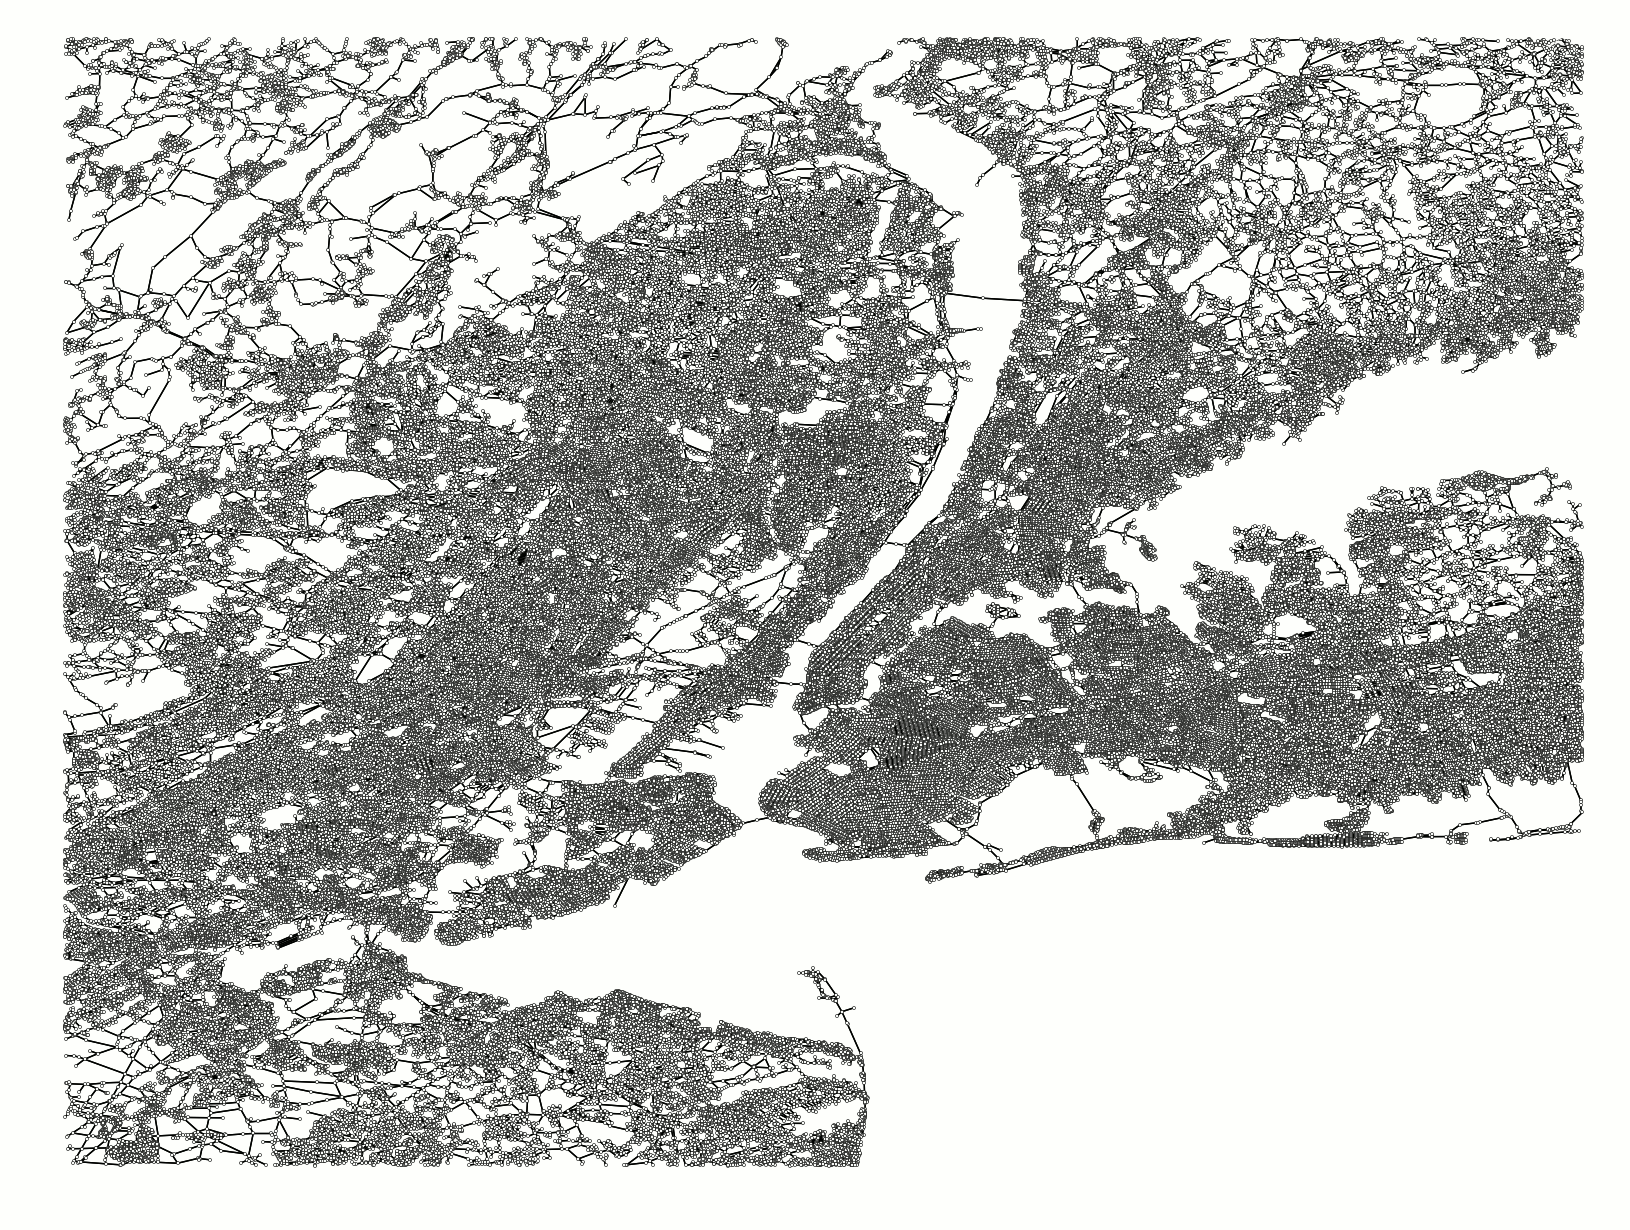
\includegraphics[width=0.8\textwidth]{NY.png}
	\caption{Representation of the New York Road Network}
	\label{fig:NewYork}
\end{figure}

For this last test, we used the road network of New York $G_{NY}$ shown in figure \ref{fig:NewYork}. This graph has about $240.000$ nodes and $730.000$ edges. We labeled the graph randomly and ran the algorithm for different regular expressions.\\

Table \ref{table:ny} shows the average running times of algorithm \ref{alg:reconsp} for REG-ShP (with implicit product network representation) and of the shortest path algorithm. The column 'Regular Exp.' shows the regular expression used for the queries, 'Time REG-ShP' is the time used to compute the regular language constrained shortest path and 'Time ShP' is the time used to compute a shortest path. Additionally, 'Dist REG-ShP' and 'Dist ShP' show the path weights, respectively.

\begin{table}[H]
	\centering
	\small
	\setlength\tabcolsep{2pt}
	\begin{tabular}{|l|l|l|l|l|}
		\hline
		Regular Exp.      & Time REG-ShP & Dist REG-ShP  & Time ShP & Dist ShP      \\ \hline
		$(a|ab)^*$        & 4.757336     & 707981.500000 & 1.862584 & 356944.800000 \\ \hline
		$(b|bab)^*|a^*$	  & 14.437849    & 333488.500000 & 1.252421 & 289889.000000 \\ \hline
		$(a|b)^*b(a|b)^2$ & 81.474183    & 406496.700000 & 1.511589 & 405458.600000 \\ \hline
	\end{tabular}
	\caption{REG-ShP on NY road network}
	\label{table:ny}
\end{table}

Here we can clearly see that the running time is strongly dependent on the regular expression. Thereby, it only matters how many production rules the equivalent NFA has and not how restrictive it is. This can be seen in the last row of the table, where the weights of the shortest and the constrained path are only slightly different but the running time is very high. 

\newpage

\section{Extensions}
\label{sec:ext}

We briefly discuss extensions of our results to language-constrained path problems. Many of these applications can be solved with dynamic-programming-based methods. But our aim is to apply the general methodology and the algorithms proposed in this thesis.\\

\subsection{Node Labels and Trip Chaining}

As a first extension, we are given a graph with node labels instead of edge labels. Now, the label of a path is defined as the concatenation of the node labels on that path. A simple transformation of the input shows that all results we developed for edge-labeled networks also hold for node-labeled networks. We transform the graph by doing the following steps: Given the (node-labeled) graph $G$ we label all edges of $G$ with a new symbol. Then, we add an additional loop to each node of $G$. This loop is labeled with the label of the corresponding node and has weight zero. The language needs to be extended such that every second symbol of a word has to be the new symbol and the word without the edge symbols is in the original language. Regular and context-free languages are closed under this operation. So we have shown that we can transfer our easiness results for edge-labeled networks to node-labeled networks.

\begin{example}
	Figure \ref{fig:nodelabels} shows a graph with node labels and its transformation to a graph with edge labels. 
\end{example}

\begin{figure}[h]
	\centering
	\begin{tikzpicture}
	[scale=.6,auto=middle,every node/.style={circle, draw}]
	\node[label={[yshift=0cm]\small $a$}] (n1) at (0,4) {$v_1$};
	\node[label={[yshift=0cm]\small $b$}] (n2) at (4,4) {$v_2$};
	\node[label={[yshift=-1.3cm]\small $b$}] (n3) at (0,0) {$v_3$};
	\node[label={[yshift=-1.3cm]\small $a$}] (n4) at (4,0) {$v_4$};
	
	\draw[->] (n1) -- (n2) node [midway, above=-4pt, draw=none] {\small 18};
	\draw[->] (n3) -- (n4) node [midway, above=-4pt, draw=none] {\small 12};
	\draw[->] (n1) -- (n3) node [midway, above=-4pt, sloped, draw=none] {\small 21};
	\draw[->] (n2) -- (n4) node [midway, above=-4pt, sloped, draw=none] {\small 23};
	\end{tikzpicture}
	
	\vspace{1em}
	
	\begin{tikzpicture}
	[scale=.6,auto=middle,every node/.style={circle, draw}]
	\node (n1) at (0,4) {$v_1$};
	\node (n2) at (4,4) {$v_2$};
	\node (n3) at (0,0) {$v_3$};
	\node (n4) at (4,0) {$v_4$};
	
	\draw[->] (n1) -- (n2) node [midway, above=-8pt, draw=none] {\small 18, $\xi$};
	\draw[->] (n3) -- (n4) node [midway, above=-8pt, draw=none] {\small 12, $\xi$};
	\draw[->] (n1) -- (n3) node [midway, above=-8pt, sloped, draw=none] {\small 21, $\xi$};
	\draw[->] (n2) -- (n4) node [midway, above=-8pt, sloped, draw=none] {\small 23, $\xi$};
	
	\path
		(n1) edge[loop above] node [midway, above=-7pt, draw=none] {\small 0, $a$} (n1)
		(n2) edge[loop above] node [midway, above=-7pt, draw=none] {\small 0, $b$} (n2)
		(n3) edge[loop below] node [midway, below=-4pt, draw=none] {\small 0, $b$} (n3)
		(n4) edge[loop below] node [midway, below=-4pt, draw=none] {\small 0, $a$} (n4);
	\end{tikzpicture}
	\caption{Transforming node labels to edge labels}
	\label{fig:nodelabels}
\end{figure}

For modeling problems related to transportation node labels turn out to be rather useful. Consider a set of activities that need to be executed in a particular order but each activity can be performed at several locations. Find a shortest path that visits one location for each activity in the given order. For instance, we might look for a shortest path from A to B, but with the condition that it visits some locations, e.g., supermarket, post office, and police station. Those locations need to be visited in this order, but with the freedom to choose one of the supermarkets, etc. in the city. Problems of this type are called trip chaining problems. They cannot be solved by a direct application of Dijkstra’s algorithm to find best paths between two consecutive subdestinations and concatenating these paths. But by assigning each location type a node label and constructing a simple regular expression, we can select locations for the subdestinations and find shortest paths in graphs that satisfy the constraints using the results proposed here.

\subsection{Left-turn and U-turn Penalties}

Another common problem of vehicle routing is known as turn penalties. Thereby taking certain left turns causes additional cost or is not desired at all. For instance, left turns can be prohibited by setting the cost to $\infty$.\\

To solve this problem we look for a shortest path in a modified network. (We reduce the given problem by replacing each intersection by a clique of size 4. This is marginally more complicated for directed networks.) The problem is varied by searching a path in which no more than $k$ left turns occur instead of giving penalties to certain turns. Dijkstra's algorithm cannot be used to solve this variant, but we can efficiently solve it using our results for language-constrained path problems. To apply these methods the road network needs to be modified. Each intersection is replaced by a clique of size 4 and labels are added to each edge. Then an automaton is constructed which accepts all words containing at most $k$ labels corresponding to left turns. This construction can be done along the lines of the $k$-similar path problem. All remaining details are easy. As an example, suppose the number of allowed left turns is a small fraction of the total number of edges in the network. This can also be solved efficiently since it can be described as a CFG.

\subsection{Time-dependent Networks}

In many applications of vehicle routing edge weights are time-dependent. A function describes the weight of each edge for a given point of time. There are several approaches for finding shortest paths in such networks. The basic idea is to use dynamic programming on functions. The corresponding algorithm combined with the results of this thesis yields a polynomial-time algorithm for CFG-ShP in time-depending networks.

\subsection{Multicriteria Shortest Paths}

As a final application, we take a look at bicriteria and multicriteria shortest path problems. In such a scenario, there might be two (or more) weight functions. For example, one specifying the cost of traveling that edge and one assigning the time it takes to traverse the edge. We aim to find a path from $s$ to $t$ with minimum cost and, additionally, the time it takes to travel the edges on that path does not exceed a given budget $B$. Many papers already discussed this problem as the resource-constrained shortest path problem (RCSP). We briefly mentioned it in section \ref{sec:found:app}. Solving the language-constrained bicriteria shortest path problem can easily be done by a polynomial-time approximation scheme since the product network simply consists out of multiple copies of the original graph. This is achieved by combining the ideas proposed here and the ones designed for used for designing approximation schemes for the basic bicriteria problem.

\newpage

\section{Conclusion}
\label{sec:conclusion}

In this thesis, we studied a variety of problems that aim to find path satisfying certain formal-language constraints. A general approach on how to efficiently model and solve such problems was presented. It turned out that the model was particularly useful in describing, understanding and solving vehicle routing problems. We described how to solve REG-ShP by constructing a product network out of a graph and an NFA. Additionally, we showed how to avoid an explicit representation of this product NFA to improve the running time of the algorithm. Furthermore, several techniques to speed up point-to-point queries were proposed. We also presented how to solve CFG-ShP and REG-SiP. Moreover, various special cases of languages or graphs were considered and several ideas for efficient algorithms were given.\\ 

In the practical part of this thesis, all algorithms were properly implemented and empirically tested. Thereby, a variety of random networks and graphs were used to obtain a broad spectrum of results. Many experiments were executed to study the performance of our algorithm for the formal-language constrained shortest path problem using various languages. By varying the underlying language, the graph classes or the considered path we obtained comprehensive results that provide a fairly tight characterization of the running time and complexity of these problems.\\

A number of questions for further investigation are raised. Some of the most interesting questions that we have left open and are hopefully able to address in future work are:

\begin{enumerate}
	\item It would be of interest to characterize the class of fixed regular languages for which the regular-language-constrained simple path problems are solvable in polynomial time.
	
	\item Implementation and basic comparison of speed-up techniques, such as the Bidirectional and the Goal-Directed Search.
\end{enumerate}

\newpage

\section*{Acknowledgments}
\label{sec:acknowledge}

I would like to express my gratitude to all those who made it possible for me to complete this thesis. I express thanks to my supervisor Prof. Dr. Sven O. Krumke for the professional support, for his assistance and for his time.\\

Furthermore, I would like to show my great appreciation to my fellow students Lena Schwehm and Jens-Peter Joost, with whom I worked on a previous project on shortest paths that built the basis for this thesis. It also motivated me to investigate and study more problems and aspects of graph theory, especially shortest path problems.\\

Special thanks go to Lisa M\"uller, Oliver Bachtler, Alexander Haag, and Marcel Sch\"utz who examined the final version of the thesis closely for English style and grammar.

\newpage

\begin{thebibliography}{Lam00}
	\bibitem[BJM00]{BJM00}
	C. Barret, R. Jacob, and M. V. Marathe,
	\emph{Formal-language-constrained path problems},
	SIAM Journal on Computing 30 (2000), no. 3, 809–837.
	
	\bibitem[BB+08]{BB+08}
	C. Barret, K. Bisset, M. Holzer, G. Konjevod, M. Marathe and D. Wagner,
	\emph{Engineering Label-Constrained Shortest-Path Algorithms},
	Algorithmic Aspects in Information and Management: 4th International Conference, AAIM (2008), 27-37.
	
	\bibitem[HT86]{HT86}
	R. Hassin and A. Tamir,
	\emph{Efficient Algorithms for Optimization and Selection on Series-Parallel Graphs},
	SIAM. J. on Algebraic and Discrete Methods, 7(3), 379–389.
	
	\bibitem[WWB08]{WWB08}
	Charles B. Ward, Nathan M. Wiegand and Phillip G. Bradford,
	\emph{A Distributed Context-Free Language Constrained Shortest Path Algorithm},
	37th International Conference on Parallel Processing (2008), 373-380.
	
	\bibitem[JBM99]{JBM99}
	R. Jacob, C. Barrett, and M. Marathe,
	\emph{Models and efficient algorithms for class of routing problems in time dependent and labeled networks},
	Technical report, Los Alamos National Laboratory, Los Alamos, NM, (1999).
	
	\bibitem[Amo93]{Amo93}
	Ravindra K. Ahuja, Thomas L. Magnanti and James B. Orlin, 
	\emph{Network Flows: Theory, Algorithms and Applications}, 
	Prentice-Hall, Englewood Cliffs, NJ (1993).
	
	\bibitem[HY87]{HY87}
	X. He and Y. Yesha,
	\emph{Parallel recognition and decomposition of two terminal series parallel graphs},
	Information and Computation 75 (1987), 15-38
	
	\bibitem[Bo2]{Bo92}
	H. L. Bodlaender,
	\emph{A tourist guide through treewidth},
	Technical report RUU-CS-92-12, Utrecht University, The Netherlands (1992).
	
	\bibitem[AV99]{AV99}
	S. Abiteboul and V. Vianu,
	\emph{Regular path queries with constraints},
	J. Comput. System Sci., 58 (1999), pp. 428–452.
	
	\bibitem[KN12]{KN12}
	Sven O. Krumke, Hartmut Noltemeier,
	\emph{Graphentheoretische Konzepte und Algorithmen},
	B. G. Teubner (2012), no. 3.
	
	\bibitem[Die06]{Die06}
	Reinhard Diestel,
	\emph{Graph Theory},
	Springer (2006), no. 3.
	
	\bibitem[ID05]{ID05}
	S. Irnich and G. Desaulniers,
	\emph{Shortest Path Problems with Resource Constraints},
	Column Generation (2005), 33-65
	
	\bibitem[ALS91]{ALS91}
	S. Arnborg, J. Lagergren, and D. Seese,
	\emph{Easy problems for tree-decomposable graphs},
	J. Algorithms, 12 (1991), pp. 308–340.
	
	\bibitem[Ha92]{Ha92}
	R. Hassin,
	\emph{Approximation schemes for the restricted shortest path problem},
	Math. Oper. Res., 17 (1992), pp. 36–42.
	
	\bibitem[BB+02]{BB+02}
	C. Barrett, K. Bisset, R. Jacob, G. Konjevod and M. Marathe,
	\emph{Classical and contemporary shortest path problems in road networks: Implementation and experimental analysis of the TRANSIMS router},
	Proc. ESA 2002, LNCS 2461, pp. 126–138, 2002.
	
	\bibitem[HMU06]{HMU06}
	J.E. Hopcroft, R. Motwani and J.D. Ullman,
	\emph{Introduction to Automata Theory, Languages, and Computation},
	Addison–Wesley, Reading, MA, (2006)
	
	\bibitem[Sch08]{Sch08}
	U. Sch\"oning,
	\emph{Theoretische Informatik - kurz gefasst},
	Spektrum Akademischer Verlag (2008)
	
	\bibitem[HRS76]{HRS76}
	H. B. Hunt III, D. Rosenkrantz, and T. Szymanski,
	\emph{On the equivalence, containment	and covering problems for regular and context free grammars},
	J. Comput. System Sci., 12 (1976), pp. 222–268.
	
	\bibitem[Str94]{Str94}
	H. Straubing,
	\emph{Finite Automata, Formal Logic, and Circuit Complexity},
	Progr. Theoret.	Comput. Sci., Birkh\"auser Boston, Boston, MA (1994).
	
	\bibitem[SJH03]{SJH03}
	H. D. Sherali, C. Jeenanunta, and A. G. Hobeika, \emph{Time-dependent, label-constrained shortest path problems with applications},
	Transportation Science,	37(3):278–293 (2003).
	
	\bibitem[SJH06]{SJH06}
	H. D. Sherali, C. Jeenanunta, and A. G. Hobeika,
	\emph{The approach-dependent, time-dependent, label-constrained shortest path problems},
	Networks, 48(2):57–67 (2006).

	
\end{thebibliography}

\newpage

\pagestyle{empty}

% Abbildungsverzeichnis
\listoffigures

% Tabellenverzeichnis
\listoftables

\newpage

\vspace*{8cm}


\section*{Declaration of Authorship}

I hereby confirm that I have written the accompanying thesis by myself, without contributions from any sources other than those cited in the text and acknowledgements. This applies also to all graphics, drawings, maps and images included in the thesis.

This thesis was not previously presented to another examination board and has not been published. \\[2ex] 

\noindent Kaiserslautern, the 9$^{th}$ of August 2016
\begin{flushright}
	% Unterschrift (handgeschrieben)
	$\overline{~~~~~~~~~\mbox{(Felix Hoffmann)}~~~~~~~~~}$
\end{flushright}


\newpage

\begin{appendices}
\setcounter{table}{0}
\renewcommand{\thetable}{B\arabic{table}}
\captionsetup[figure]{list=no}
\captionsetup[table]{list=no}

\section{Source Code}
\label{app:code}

\begin{lstlisting}
class Automaton:

	@staticmethod
	def graph_to_automaton(G, sources, targets):
		"""Coverts graph G to equivalent NFA.
		Parameters:
		G : NetworkX graph
		sources : list of nodes (Starting nodes)
		targets : list of nodes (Ending nodes)
		
		Returns:
		automaton : FAdo NFA (NFA representing graph G)"""

	@staticmethod
	def automaton_to_graph(automaton):
		"""Coverts NFA automaton to equivalent graph G.
		Parameters:
		automaton : FAdo NFA
		
		Returns:
		G : NetworkX graph (Graph representing NFA automaton)
		sources : list of nodes (Starting nodes)
		targets : list of nodes (Ending nodes)"""
	
	@staticmethod
	def regex_to_automaton(regex_str):
		"""Coverts graph G to equivalent NFA.
		Parameters:
		regex_str : string (representing regular expression)
		
		Returns:
		automaton : FAdo NFA (NFA for regular expression)"""
	
	@staticmethod
	def product_automaton(weighted_automaton, other_automaton):
		"""Computes product of NFA and DFA.
		Parameters:
		weighted_automaton : FAdo NFA
		other_automaton : FAdo DFA
		
		Returns:
		automaton : FAdo NFA (product NFA of weighted_automaton
		and	other_automaton)"""


class BinHeap:

	def __init__(self):
		"""Initialize a binary heap."""
	
	def bubbleUp(self, i):
		"""Restores heap property by traversing up.
		Parameters:
		i : int (index of element to bubble up)"""
	
	def insert(self, element, key):
		"""Inserts element into the heap
		Parameters:
		element : (element to insert into heap)
		key : int (key value of element)"""
	
	def bubbleDown(self, i):
		"""Restores heap property by traversing down
		Parameters:
		i : int (index of element to bubble down)"""
	
	def minChild(self, i):
		"""Computes child of element i with minimum key value
		Parameters:
		i : int (index of element)
		
		Returns:
		: int (index of minimum child)"""
	
	def extractMin(self):
		"""Computes element i with minimum key value
		Returns:
		min : (element with min key value)"""
	
	def decreaseKey(self, element, key):
		"""Decreases key of element in the heap
		Parameters:
		element : (element to decrease key from)
		key : int (new key value)"""


class REGLanguage:

	@staticmethod
	def st_reg_shortest_path__product_nfa(G, source, target,
	regex_str, timeit=False):
		"""Computes regular language constrained shortest path
		from source	to target in the graph.
		Parameters:
		G : NetworkX graph
		source : node (Starting node for path)
		target : node (Ending node for path)
		regex_str : string (specifies regular expression)
		timeit : bool, optional (default = False; If True
		running time is returned)
		
		Returns:
		dist : int (The length of the shortest path)
		path : list (A list of nodes in the shortest path)
		times : dictionary (dictionary with running times)"""
	
	@staticmethod
	def st_reg_shortest_path(G, source, target, regex_str,
	timeit=False):
		"""Computes regular language constrained shortest path
		from source	to target in the graph.
		Parameters:
		G : NetworkX graph
		source : node (Starting node for path)
		target : node (Ending node for path)
		regex_str : string (specifies regular expression)
		timeit : bool, optional (default = False; If True
		running	time is returned)
		
		Returns:
		dist : int (The length of the shortest path)
		path : list (A list of nodes in the shortest path)
		times : dictionary (dictionary with running times)"""


class CFLanguage:

	@staticmethod
	def initialize_matrix(G, grammar):
		"""Initializes table D for cfl-constrained all-pair
		shortest path algorithm.
		Parameters:
		G : NetworkX graph
		grammar: FAdo CNF (grammar in Chomskey Normal From)
		
		Returns:
		D : dictionary (Table with initial distance values)"""
	
	@staticmethod
	def all_pair_cfg_shortest_path(G, grammar):
		"""Computes context-free language constrained all-pair
		shortest paths in the graph.
		Parameters:
		G : NetworkX graph
		grammar: FAdo CNF (grammar in Chomskey Normal From)
		
		Returns:
		D : dictionary (Table with shortest-path distances)"""


class KSimilarPath:

	@staticmethod
	def st_k_similar_path(G, source, target, k):
		"""Computes k-similar path in the graph G.
		Parameters:
		G : NetworkX graph
		source : node (Starting node for paths)
		target : node (Ending node for paths)
		k : int (number of common edges allowed)
		
		Returns:
		dist : int (The length of the shortest path)
		distk : int (The length of the k-similar path)
		path : list (A list of nodes in the shortest path)
		pathk : list (A list of nodes in the k-similar path)"""


class GrammarHelper:

	@staticmethod
	def is_derivable(grammar, word):
		"""Tests if word is accepted by grammar.
		Parameters:
		grammar: FAdo CNF (grammar in Chomskey Normal From)
		word : list (list of terminal symbols)
		
		Returns:
		: bool (whether word is derivable)"""
	
	@staticmethod
	def get_derivatives_of(grammar, nonterminal):
		"""Computes derivatives of nonterminal.
		Parameters:
		grammar: FAdo CNF (grammar in Chomskey Normal From)
		nonterminal : string (nonterminal symbol of grammar)
		
		Returns:
		derivatives : set"""


class GraphGenerator:

	@staticmethod
	def random_weighted_graph(number_of_nodes, p, max_weight):
		"""Generates random weighted directed graph.
		Parameters:
		number_of_nodes: int (number of nodes in the graph)
		p : float (probability for edges in the graph)
		max_weight : int (maximum weight for edges)
		
		Returns:
		G : NetworkX graph"""
		
	@staticmethod
	def random_weighted_dag(number_of_nodes, p, max_weight):
		"""Generates random weighted directed acyclic graph.
		Parameters:
		number_of_nodes: int (number of nodes in the graph)
		p : float (probability for edges in the graph)
		max_weight : int (maximum weight for edges)
		
		Returns:
		DAG : NetworkX graph"""	
	
	@staticmethod
	def random_weighted_spg(number_of_edges, max_weight):
		"""Generates random weighted directed acyclic graph.
		Parameters:
		number_of_edges: int (number of edges in the graph)
		max_weight : int (maximum weight for edges)
		
		Returns:
		SPG : NetworkX graph"""	
	
	@staticmethod
	def random_weighted_labeled_grid(m, n, max_weight, sigma):
		"""Generates random weighted labeled grid graph.
		Parameters:
		m: int (number of rows of the grid)
		n: int (number of columns of the grid)
		max_weight : int (maximum weight for edges)
		sigma : list (alphabet for labels)
		
		Returns:
		G : NetworkX graph
		dic: dictionary (positions of the nodes)"""
	
	@staticmethod
	def random_road_network(m, n, max_weight, sigma):
		"""Generates random weighted labeled road network.
		Parameters:
		m: int (number of rows of the grid)
		n: int (number of columns of the grid)
		max_weight : int (maximum weight for edges)
		sigma : list (alphabet for labels)
		
		Returns:
		G : NetworkX graph
		dic: dictionary (positions of the nodes)"""
	
	@staticmethod
	def random_label(G, sigma):
		"""Randomly labels edges on graph.
		Parameters:
		G : NetworkX graph
		sigma : list (alphabet for labels)
		
		Returns:
		G : NetworkX graph"""


class GraphHelper:

	@staticmethod
	def get_all_nodes_in_rectangle(dic, x1, x2, y1, y2):
		"""Computes all nodes in specified rectangle.
		Parameters:
		dic: dictionary (positions of the nodes)
		x1, x2, y1, y2 : int (interval borders)
		
		Returns:
		L : list (list of nodes)"""
	
	@staticmethod
	def get_rectangle_around_s_and_t(dic, source, target,
	path=None):
		"""Computes all nodes in rectangle around source and target.
		Parameters:
		dic: dictionary (positions of the nodes)
		source, target : node
		path : list, optional (default = None)
		
		Returns:
		L : list (list of nodes)"""
	
	@staticmethod
	def make_graph_geometric(G, dic):
		"""Computes geometric distance for edge weights.
		Parameters:
		G : NetworkX graph
		dic: dictionary (positions of the nodes)
		
		Returns:
		G : NetworkX graph"""
	
	@staticmethod
	def merge_nodes(G, selected_nodes, new_node):
		"""Merges selected_nodes into new_node.
		Parameters:
		G : NetworkX graph
		selected_nodes : list (nodes to merge)
		new_node : (node to merge to)
		
		Returns:
		G : NetworkX graph"""
	
	@staticmethod
	def get_edgelist_from_nodelist(nodelist):
		"""Computes edgelist from nodelist.
		Parameters:
		nodelist : list (list of connected nodes)
		
		Returns:
		edgelist : list (list of edges)"""
	
	@staticmethod
	def get_nodelist_from_edgelist(edgelist):
		"""Computes nodelist from edgelist.
		Parameters:
		edgelist : list (list of adjacent edges)
		
		Returns:
		nodelist : list (list of nodes)"""
	
	@staticmethod
	def get_lables_from_nodelist(G, nodelist):
		"""Computes labels of nodelist.
		Parameters:
		nodelist : list (list of connected nodes)
		
		Returns:
		word : str (concatenated labels of nodelist)"""
	
	@staticmethod
	def convert_node_labels_to_integers(G, pos):
		"""Converts node labels to integers.
		Parameters:
		G : NetworkX graph
		pos: dictionary (positions of the nodes)
		
		Returns:
		G : NetworkX graph
		new_pos: dictionary (positions of the nodes)"""


class Reader:

	@staticmethod
	def convert_to_graph(filename):
		"""Reads graph from file(s).
		Parameters:
		filename : string (i.e.: "USA-road-d.NY")
		
		Returns:
		G : NetworkX graph
		dic: dictionary (positions of the nodes)"""
	
	@staticmethod
	def get_graph_data(filename):
		"""Reads graph from file.
		Parameters:
		filename : string (filename of gr-file)
		
		Returns:
		G : NetworkX graph"""
	
	@staticmethod
	def get_coordinates(filename):
		"""Reads node coordinates from file.
		Parameters:
		filename : string (filename of co-file)
		
		Returns:
		dic: dictionary (positions of the nodes)"""


class Dijkstra:

	@staticmethod
	def s_shortest_path(G, source):
		"""Computes shortest path from source to all nodes in the
		graph G.
		Parameters:
		G : NetworkX graph
		source : node (Starting node for path)
		
		Returns:
		dist: dict (dictionary of shortest path distances)
		pred: dict (dictionary of predecessors)"""
	
	@staticmethod
	def s_shortest_path_heap(G, source):
		"""Computes shortest path from source to all nodes in the
		graph G using a heap as priority list.
		Parameters:
		G : NetworkX graph
		source : node (Starting node for path)
		
		Returns:
		dist: dict (dictionary of shortest path distances)
		pred: dict (dictionary of predecessors)"""
	
	@staticmethod
	def st_shortest_path_heap(G, source, target):
		"""Computes shortest path from source to target in the
		graph G using a heap as priority list.
		Raises NetworkXNoPath exception when no path exists.
		Parameters:
		G : NetworkX graph
		source : node (Starting node for path)
		target : node (Ending node for path)
		
		Returns:
		dist: int (The length of the shortest path)
		path: list (A list of nodes in the shortest path)"""

	
class DAGraph:
	
	@staticmethod
	def top_sort(G):
		"""Computes topological sorting of DAG G.
		Parameters:
		G : NetworkX graph
		
		Returns:
		graph_sorted: list (nodes in topological sort order)"""
	
	@staticmethod
	def s_shortest_path(G, source):
		"""Computes shortest path in the directed acyclic graph G.
		Parameters:
		G : NetworkX graph
		source : node (Starting node for path)
		
		Returns:
		dist: dict (dictionary of shortest path distances)
		pred: dict (dictionary of predecessors)"""
	
	
class SPGraph:
	
	@staticmethod
	def st_shortest_path(G, source, target):
		"""Computes shortest path in the series-parallel graph G.
		Parameters:
		G : NetworkX graph
		source : node (Starting node for path)
		target : node (Ending node for path)
		
		Returns:
		dist: int (The length of the shortest path)
		path: list (A list of nodes in the shortest path)"""
\end{lstlisting}

\clearpage

\section{Tables}
\label{app:tables}

\subsection{Tables for REG-ShP}
\label{app:tables:reg}

Full tables from section \ref{sec:study:reg}.\\

\begin{table}[H]
	\centering
	\small
	\setlength\tabcolsep{2pt}
	\begin{tabular}{|l|l|l|l|l|}
		\hline
		N     & Total Time & Regex to NFA & Pre-Processing & Calculate Path \\ \hline
		25    & 0.001756   & 0.001487     & 0.000079       & 0.000190       \\ \hline
		100   & 0.002722   & 0.001494     & 0.000303       & 0.000925       \\ \hline
		225   & 0.004576   & 0.001521     & 0.000671       & 0.002384       \\ \hline
		400   & 0.007325   & 0.001608     & 0.001405       & 0.004311       \\ \hline
		625   & 0.011612   & 0.001705     & 0.002418       & 0.007489       \\ \hline
		900   & 0.015810   & 0.001822     & 0.003695       & 0.010292       \\ \hline
		1600  & 0.030691   & 0.001933     & 0.007027       & 0.021731       \\ \hline
		2500  & 0.047557   & 0.001927     & 0.012045       & 0.033585       \\ \hline
		3600  & 0.078203   & 0.001918     & 0.017171       & 0.059114       \\ \hline
		5625  & 0.117096   & 0.002014     & 0.032214       & 0.082869       \\ \hline
		10000 & 0.239353   & 0.002016     & 0.057503       & 0.179834       \\ \hline
	\end{tabular}
	\caption{REG-ShP with implicit representation, $R = (a|ab)^*$}
\end{table}

\begin{table}[H]
	\centering
	\small
	\setlength\tabcolsep{2pt}
	\begin{tabular}{|l|l|l|l|l|}
		\hline
		N     & Total Time & Regex to NFA & Product NFA & Calculate Path \\ \hline
		25    & 0.002050   & 0.001641     & 0.000236    & 0.000173       \\ \hline
		100   & 0.004522   & 0.002183     & 0.001506    & 0.000834       \\ \hline
		225   & 0.009670   & 0.003245     & 0.004296    & 0.002129       \\ \hline
		400   & 0.020896   & 0.005184     & 0.011812    & 0.003900       \\ \hline
		625   & 0.038729   & 0.008050     & 0.023969    & 0.006711       \\ \hline
		900   & 0.066927   & 0.012753     & 0.045171    & 0.009002       \\ \hline
		1600  & 0.176817   & 0.028323     & 0.129295    & 0.019199       \\ \hline
		2500  & 0.404677   & 0.057987     & 0.317109    & 0.029581       \\ \hline
		3600  & 0.767475   & 0.102163     & 0.615390    & 0.049921       \\ \hline
		5625  & 1.862021   & 0.240999     & 1.548801    & 0.072221       \\ \hline
		10000 & 5.522037   & 0.686569     & 4.680135    & 0.155333       \\ \hline
	\end{tabular}
	\caption{REG-ShP with product NFA, $R = (a|ab)^*$}
\end{table}

\begin{table}[H]
	\centering
	\small
	\setlength\tabcolsep{2pt}
	\begin{tabular}{|l|l|l|l|l|}
		\hline
		N     & Total Time & Regex to NFA & Pre-Processing & Calculate Path \\ \hline
		25    & 0.003538   & 0.001665     & 0.000082       & 0.001792       \\ \hline
		100   & 0.011548   & 0.001730     & 0.000310       & 0.009509       \\ \hline
		225   & 0.024205   & 0.001879     & 0.000737       & 0.021589       \\ \hline
		400   & 0.046162   & 0.002031     & 0.001548       & 0.042584       \\ \hline
		625   & 0.080005   & 0.002057     & 0.002779       & 0.075169       \\ \hline
		900   & 0.115618   & 0.002055     & 0.003749       & 0.109814       \\ \hline
		1600  & 0.210226   & 0.002079     & 0.007242       & 0.200904       \\ \hline
		2500  & 0.357855   & 0.002066     & 0.010735       & 0.345054       \\ \hline
		3600  & 0.544368   & 0.002066     & 0.020820       & 0.521482       \\ \hline
		5625  & 0.861782   & 0.002130     & 0.027414       & 0.832238       \\ \hline
		10000 & 1.562226   & 0.002198     & 0.052075       & 1.507953       \\ \hline
	\end{tabular}
	\caption{REG-ShP with implicit representation, $R = (b|bab)^*|a^*$}
\end{table}

\begin{table}[H]
	\centering
	\small
	\setlength\tabcolsep{2pt}
	\begin{tabular}{|l|l|l|l|l|}
		\hline
		N     & Total Time & Regex to NFA & Product NFA & Calculate Path \\ \hline
		25    & 0.003969   & 0.001801     & 0.000557    & 0.001611       \\ \hline
		100   & 0.015588   & 0.002386     & 0.004648    & 0.008555       \\ \hline
		225   & 0.041558   & 0.003510     & 0.018740    & 0.019308       \\ \hline
		400   & 0.092949   & 0.005433     & 0.049237    & 0.038279       \\ \hline
		625   & 0.192100   & 0.008274     & 0.115894    & 0.067933       \\ \hline
		900   & 0.342928   & 0.012825     & 0.232022    & 0.098082       \\ \hline
		1600  & 0.924148   & 0.028145     & 0.719016    & 0.176987       \\ \hline
		2500  & 2.090122   & 0.070942     & 1.720379    & 0.298801       \\ \hline
		3600  & 4.068409   & 0.103436     & 3.504668    & 0.460305       \\ \hline
		5625  & 9.345573   & 0.242839     & 8.365048    & 0.737687       \\ \hline
		10000 & 28.402813  & 0.670863     & 26.391114   & 1.340837       \\ \hline
	\end{tabular}
	\caption{REG-ShP with product NFA, $R = (b|bab)^*|a^*$}
\end{table}

\begin{table}[H]
	\centering
	\small
	\setlength\tabcolsep{2pt}
	\begin{tabular}{|l|l|l|l|l|}
		\hline
		N     & Total Time & Regex to NFA & Pre-Processing & Calculate Path \\ \hline
		25    & 0.001864   & 0.001593     & 0.000074       & 0.000197       \\ \hline
		100   & 0.002523   & 0.001754     & 0.000384       & 0.000385       \\ \hline
		225   & 0.003736   & 0.001832     & 0.000915       & 0.000990       \\ \hline
		400   & 0.004093   & 0.001784     & 0.001615       & 0.000694       \\ \hline
		625   & 0.005036   & 0.001798     & 0.002518       & 0.000720       \\ \hline
		900   & 0.006340   & 0.001832     & 0.003622       & 0.000887       \\ \hline
		1600  & 0.010156   & 0.002007     & 0.006971       & 0.001179       \\ \hline
		2500  & 0.015692   & 0.002054     & 0.012201       & 0.001437       \\ \hline
		3600  & 0.023018   & 0.002130     & 0.018928       & 0.001960       \\ \hline
		5626  & 0.051947   & 0.003089     & 0.043457       & 0.005401       \\ \hline
		10000 & 0.076837   & 0.002463     & 0.068647       & 0.005728       \\ \hline
	\end{tabular}
	\caption{REG-ShP with implicit representation, $R = a^*((b|cd)^*|e)$}
\end{table}

\begin{table}[H]
	\centering
	\small
	\setlength\tabcolsep{2pt}
	\begin{tabular}{|l|l|l|l|l|}
		\hline
		N     & Total Time & Regex to NFA & Product NFA & Calculate Path \\ \hline
		25    & 0.002289   & 0.001734     & 0.000357    & 0.000198       \\ \hline
		100   & 0.005775   & 0.002426     & 0.002951    & 0.000398       \\ \hline
		225   & 0.016204   & 0.003784     & 0.011459    & 0.000962       \\ \hline
		400   & 0.036927   & 0.005440     & 0.030769    & 0.000718       \\ \hline
		625   & 0.078702   & 0.008497     & 0.069412    & 0.000793       \\ \hline
		900   & 0.151972   & 0.012749     & 0.138214    & 0.001008       \\ \hline
		1600  & 0.470986   & 0.027948     & 0.441573    & 0.001465       \\ \hline
		2500  & 1.116766   & 0.053672     & 1.061411    & 0.001683       \\ \hline
		3600  & 2.310253   & 0.099937     & 2.208236    & 0.002080       \\ \hline
		5626  & 7.237197   & 0.292584     & 6.939044    & 0.005569       \\ \hline
		10000 & 19.920313  & 0.707659     & 19.207002   & 0.005652       \\ \hline
	\end{tabular}
	\caption{REG-ShP with product NFA, $R = a^*((b|cd)^*|e)$}
\end{table}

\begin{table}[H]
	\centering
	\small
	\setlength\tabcolsep{2pt}
	\begin{tabular}{|l|l|l|l|l|}
		\hline
		N     & Total Time & Regex to NFA & Pre-Processing  & Calculate Path    \\ \hline
		25    & 0.001827   & 0.001495     & 0.000077        & 0.000256  		\\ \hline
		100   & 0.003071   & 0.001609     & 0.000314        & 0.001147  		\\ \hline
		225   & 0.004766   & 0.001603     & 0.000667        & 0.002496  		\\ \hline
		400   & 0.007720   & 0.001741     & 0.001527        & 0.004453  		\\ \hline
		625   & 0.012834   & 0.001835     & 0.002572        & 0.008427  		\\ \hline
		900   & 0.018826   & 0.001880     & 0.003328        & 0.013617  		\\ \hline
		1600  & 0.029411   & 0.001921     & 0.006158        & 0.021332  		\\ \hline
		2500  & 0.054244   & 0.001914     & 0.011979        & 0.040350  		\\ \hline
		3600  & 0.074247   & 0.001958     & 0.015205        & 0.057084  		\\ \hline
		5625  & 0.126562   & 0.002018     & 0.035990        & 0.088555  		\\ \hline
		10000 & 0.247716   & 0.002117     & 0.064475        & 0.181125  		\\ \hline
	\end{tabular}
	\caption{REG-ShP with implicit representation, $R = 0(0|1)^*1$}
\end{table}

\begin{table}[H]
	\centering
	\small
	\setlength\tabcolsep{2pt}
	\begin{tabular}{|l|l|l|l|l|}
		\hline
		N     & Total Time  & Regex to NFA & Product NFA  & Calculate Path  \\ \hline
		25    & 0.002209    & 0.001638     & 0.000343     & 0.000228        \\ \hline
		100   & 0.005771    & 0.002299     & 0.002449     & 0.001023  	    \\ \hline
		225   & 0.013764    & 0.003259     & 0.008275     & 0.002231  		\\ \hline
		400   & 0.031313    & 0.005308     & 0.022074     & 0.003931  		\\ \hline
		625   & 0.063162    & 0.008147     & 0.047580     & 0.007436  		\\ \hline
		900   & 0.115288    & 0.012484     & 0.091033     & 0.011770  		\\ \hline
		1600  & 0.318985    & 0.028185     & 0.272436     & 0.018364  		\\ \hline
		2500  & 0.740536    & 0.055964     & 0.650127     & 0.034444  		\\ \hline
		3600  & 1.463151    & 0.096320     & 1.316362     & 0.050468  		\\ \hline
		5625  & 3.457060    & 0.219723     & 3.161065     & 0.076271  		\\ \hline
		10000 & 10.608229   & 0.650123     & 9.802193     & 0.155914  		\\ \hline
	\end{tabular}
	\caption{REG-ShP with product NFA, $R = 0(0|1)^*1$}
\end{table}

\begin{table}[H]
	\centering
	\small
	\setlength\tabcolsep{2pt}
	\begin{tabular}{|l|l|l|l|l|}
		\hline
		N     & Total Time & Regex to NFA & Pre-Processing & Calculate Path  \\ \hline
		25    & 0.001950   & 0.001622     & 0.000077       & 0.000251        \\ \hline
		100   & 0.003231   & 0.001611     & 0.000295       & 0.001325        \\ \hline
		225   & 0.005463   & 0.001671     & 0.000681       & 0.003112        \\ \hline
		400   & 0.008705   & 0.001758     & 0.001366       & 0.005581        \\ \hline
		625   & 0.014215   & 0.001866     & 0.002213       & 0.010135        \\ \hline
		900   & 0.023301   & 0.001931     & 0.006588       & 0.014782        \\ \hline
		1600  & 0.034795   & 0.001977     & 0.006154       & 0.026664        \\ \hline
		2500  & 0.065601   & 0.001987     & 0.012918       & 0.050696        \\ \hline
		3600  & 0.083728   & 0.001980     & 0.016380       & 0.065368        \\ \hline
		5625  & 0.148843   & 0.002041     & 0.043475       & 0.103327        \\ \hline
		10000 & 0.319898   & 0.002007     & 0.104213       & 0.213678        \\ \hline
	\end{tabular}
	\caption{REG-ShP with implicit representation, $R = 1^*(01^*01^*)^*$}
\end{table}

\begin{table}[H]
	\centering
	\small
	\setlength\tabcolsep{2pt}
	\begin{tabular}{|l|l|l|l|l|}
		\hline
		N     & Total Time & Regex to NFA & Product NFA & Calculate Path \\ \hline
		25    & 0.002267   & 0.001770     & 0.000272    & 0.000225       \\ \hline
		100   & 0.005064   & 0.002289     & 0.001600    & 0.001175       \\ \hline
		225   & 0.010931   & 0.003536     & 0.004658    & 0.002737       \\ \hline
		400   & 0.029069   & 0.005232     & 0.018866    & 0.004971       \\ \hline
		625   & 0.048242   & 0.008006     & 0.031320    & 0.008916       \\ \hline
		900   & 0.089055   & 0.018828     & 0.058194    & 0.012032       \\ \hline
		1600  & 0.286004   & 0.094656     & 0.167721    & 0.023628       \\ \hline
		2500  & 0.463885   & 0.068692     & 0.354319    & 0.040873       \\ \hline
		3600  & 0.858608   & 0.125721     & 0.678313    & 0.054573       \\ \hline
		5625  & 1.897599   & 0.273904     & 1.534471    & 0.089224       \\ \hline
		10000 & 5.554214   & 0.690296     & 4.677283    & 0.186636       \\ \hline
	\end{tabular}
	\caption{REG-ShP with product NFA, $R = 1^*(01^*01^*)^*$}
\end{table}

\begin{table}[H]
	\centering
	\small
	\setlength\tabcolsep{2pt}
	\begin{tabular}{|l|l|l|l|l|}
		\hline
		N     & Total Time & Regex to NFA & Pre-Processing & Calculate Path  \\ \hline
		25    & 0.006797   & 0.001960     & 0.000089       & 0.004748        \\ \hline
		100   & 0.026172   & 0.002157     & 0.000319       & 0.023697        \\ \hline
		225   & 0.061174   & 0.002325     & 0.002030       & 0.056819        \\ \hline
		400   & 0.108503   & 0.002335     & 0.001586       & 0.104582        \\ \hline
		625   & 0.165595   & 0.002378     & 0.002408       & 0.160810        \\ \hline
		900   & 0.282404   & 0.002395     & 0.003639       & 0.276370        \\ \hline
		1600  & 0.469986   & 0.002373     & 0.009806       & 0.457806        \\ \hline
		2500  & 0.793235   & 0.002391     & 0.014808       & 0.776036        \\ \hline
		3600  & 1.171519   & 0.002459     & 0.016746       & 1.152314        \\ \hline
		5625  & 1.899416   & 0.002752     & 0.030665       & 1.865999        \\ \hline
		10000 & 3.901605   & 0.002909     & 0.057477       & 3.841219        \\ \hline
	\end{tabular}
	\caption{REG-ShP with implicit representation, $R = (a|b)^*b(a|b)^2$}
\end{table}

\begin{table}[H]
	\centering
	\small
	\setlength\tabcolsep{2pt}
	\begin{tabular}{|l|l|l|l|l|}
		\hline
		N     & Total Time & Regex to NFA & Product NFA & Calculate Path \\ \hline
		25    & 0.007622   & 0.002074     & 0.001369    & 0.004179       \\ \hline
		100   & 0.038351   & 0.002703     & 0.014624    & 0.021024       \\ \hline
		225   & 0.101854   & 0.003823     & 0.048110    & 0.049921       \\ \hline
		400   & 0.224002   & 0.005739     & 0.125809    & 0.092454       \\ \hline
		625   & 0.452994   & 0.009741     & 0.300538    & 0.142715       \\ \hline
		900   & 0.875571   & 0.014109     & 0.618849    & 0.242613       \\ \hline
		1600  & 2.285875   & 0.050116     & 1.833743    & 0.402015       \\ \hline
		2500  & 5.096695   & 0.060503     & 4.351700    & 0.684492       \\ \hline
		3600  & 9.898741   & 0.104680     & 8.780789    & 1.013272       \\ \hline
		5625  & 22.796797  & 0.227646     & 20.929542   & 1.639609       \\ \hline
		10000 & 72.141304  & 0.702462     & 68.093412   & 3.345430       \\ \hline
	\end{tabular}
	\caption{REG-ShP with product NFA, $R = (a|b)^*b(a|b)^2$}
\end{table}

\subsection{Tables for k-similar Path}
\label{app:tables:ksim}

Full tables from section \ref{sec:study:ksim}.\\

\begin{table}[H]
	\centering
	\small
	\setlength\tabcolsep{2pt}
	\begin{tabular}{|l|l|l|l|l|l|l|l|}
		\hline
		k  & Total Time & Time KSimP & Dist KSimP & Nodes KSimP & Time ShP & Dist ShP  & Nodes ShP \\ \hline
		0  & 0.001822   & 0.001716   & 101.370000 & 5.480000    & 0.000106 & 61.030000 & 4.340000  \\ \hline
		1  & 0.002346   & 0.002245   & 81.610000  & 4.710000    & 0.000101 & 62.930000 & 4.550000  \\ \hline
		2  & 0.003505   & 0.003405   & 69.390000  & 4.490000    & 0.000100 & 58.190000 & 4.250000  \\ \hline
		5  & 0.008348   & 0.008243   & 61.180000  & 4.220000    & 0.000105 & 60.690000 & 4.220000  \\ \hline
		10 & 0.024179   & 0.024070   & 62.830000  & 4.590000    & 0.000109 & 62.830000 & 4.590000  \\ \hline
		20 & 0.084538   & 0.084430   & 63.950000  & 4.440000    & 0.000108 & 63.950000 & 4.440000  \\ \hline
		30 & 0.182751   & 0.182646   & 60.300000  & 4.380000    & 0.000105 & 60.300000 & 4.380000  \\ \hline
		40 & 0.321416   & 0.321313   & 57.980000  & 4.340000    & 0.000102 & 57.980000 & 4.340000  \\ \hline
		50 & 0.541389   & 0.541269   & 68.770000  & 4.640000    & 0.000120 & 68.770000 & 4.640000  \\ \hline
	\end{tabular}
	\caption{K-similar Path on graph with 25 nodes}
\end{table}

\begin{table}[H]
	\centering
	\small
	\setlength\tabcolsep{2pt}
	\begin{tabular}{|l|l|l|l|l|l|l|l|}
		\hline
		k  & Total Time & Time KSimP & Dist KSimP & Nodes KSimP & Time ShP & Dist ShP   & Nodes ShP \\ \hline
		0  & 0.002957   & 0.002473   & 166.850000 & 10.470000   & 0.000483 & 114.680000 & 9.110000  \\ \hline
		1  & 0.005288   & 0.004834   & 144.040000 & 8.910000    & 0.000454 & 105.840000 & 7.890000  \\ \hline
		2  & 0.009336   & 0.008882   & 139.640000 & 9.120000    & 0.000454 & 109.190000 & 8.740000  \\ \hline
		5  & 0.031200   & 0.030733   & 124.260000 & 8.640000    & 0.000467 & 110.920000 & 8.640000  \\ \hline
		10 & 0.100238   & 0.099748   & 116.800000 & 8.830000    & 0.000490 & 114.540000 & 8.890000  \\ \hline
		20 & 0.337520   & 0.337021   & 114.340000 & 8.670000    & 0.000499 & 114.340000 & 8.590000  \\ \hline
		30 & 0.763241   & 0.762722   & 120.840000 & 9.040000    & 0.000520 & 120.840000 & 9.000000  \\ \hline
		40 & 1.369042   & 1.368542   & 110.990000 & 8.470000    & 0.000501 & 110.990000 & 8.430000  \\ \hline
		50 & 2.122464   & 2.121978   & 111.320000 & 8.330000    & 0.000486 & 111.320000 & 8.310000  \\ \hline
	\end{tabular}
	\caption{K-similar Path on graph with 100 nodes}
\end{table}

\begin{table}[H]
	\centering
	\small
	\setlength\tabcolsep{2pt}
	\begin{tabular}{|l|l|l|l|l|l|l|l|}
		\hline
		k  & Total Time & Time KSimP & Dist KSimP & Nodes KSimP & Time ShP & Dist ShP   & Nodes ShP \\ \hline
		0  & 0.005436   & 0.004190   & 242.480000 & 13.220000   & 0.001247 & 184.750000 & 12.360000 \\ \hline
		1  & 0.011220   & 0.010016   & 216.830000 & 12.380000   & 0.001204 & 174.430000 & 11.620000 \\ \hline
		2  & 0.022465   & 0.021186   & 213.100000 & 12.530000   & 0.001279 & 179.060000 & 12.270000 \\ \hline
		5  & 0.074240   & 0.073022   & 196.700000 & 12.130000   & 0.001218 & 178.160000 & 12.230000 \\ \hline
		10 & 0.226509   & 0.225349   & 173.730000 & 11.430000   & 0.001160 & 169.170000 & 11.270000 \\ \hline
		20 & 0.880579   & 0.879293   & 185.560000 & 12.490000   & 0.001286 & 185.390000 & 12.510000 \\ \hline
		30 & 1.808665   & 1.807341   & 181.610000 & 12.470000   & 0.001324 & 181.610000 & 12.430000 \\ \hline
		40 & 2.828033   & 2.826927   & 166.190000 & 10.990000   & 0.001106 & 166.190000 & 10.910000 \\ \hline
		50 & 5.070261   & 5.069027   & 185.930000 & 12.680000   & 0.001233 & 185.930000 & 12.640000 \\ \hline
	\end{tabular}
	\caption{K-similar Path on graph with 225 nodes}
\end{table}

\begin{table}[H]
	\centering
	\small
	\setlength\tabcolsep{2pt}
	\begin{tabular}{|l|l|l|l|l|l|l|l|}
		\hline
		k  & Total Time & Time KSimP & Dist KSimP & Nodes KSimP & Time ShP & Dist ShP   & Nodes ShP \\ \hline
		0  & 0.008682   & 0.006452   & 288.460000 & 17.440000   & 0.002229 & 225.900000 & 15.900000 \\ \hline
		1  & 0.017696   & 0.015686   & 248.180000 & 15.500000   & 0.002010 & 201.060000 & 14.900000 \\ \hline
		2  & 0.033923   & 0.031916   & 241.940000 & 15.180000   & 0.002007 & 203.330000 & 14.680000 \\ \hline
		5  & 0.131044   & 0.128857   & 234.410000 & 15.790000   & 0.002186 & 213.300000 & 15.410000 \\ \hline
		10 & 0.429914   & 0.427661   & 223.390000 & 15.130000   & 0.002253 & 214.320000 & 15.110000 \\ \hline
		20 & 1.426821   & 1.424657   & 217.210000 & 15.320000   & 0.002165 & 216.240000 & 15.340000 \\ \hline
		30 & 3.146463   & 3.144153   & 228.110000 & 16.370000   & 0.002310 & 228.010000 & 16.370000 \\ \hline
		40 & 4.340988   & 4.339080   & 185.310000 & 13.600000   & 0.001908 & 185.310000 & 13.480000 \\ \hline
		50 & 7.739592   & 7.737405   & 212.440000 & 15.320000   & 0.002186 & 212.440000 & 15.220000 \\ \hline
	\end{tabular}
	\caption{K-similar Path on graph with 400 nodes}
\end{table}

\begin{table}[H]
	\centering
	\small
	\setlength\tabcolsep{2pt}
	\begin{tabular}{|l|l|l|l|l|l|l|l|}
		\hline
		k  & Total Time & Time KSimP & Dist KSimP & Nodes KSimP & Time ShP & Dist ShP   & Nodes ShP \\ \hline
		0  & 0.013024   & 0.009417   & 336.610000 & 20.510000   & 0.003606 & 268.310000 & 19.190000 \\ \hline
		1  & 0.029312   & 0.025725   & 333.740000 & 21.700000   & 0.003587 & 277.760000 & 20.380000 \\ \hline
		2  & 0.058169   & 0.054555   & 307.500000 & 20.190000   & 0.003615 & 263.310000 & 19.290000 \\ \hline
		5  & 0.212769   & 0.209170   & 300.420000 & 20.420000   & 0.003600 & 268.910000 & 19.820000 \\ \hline
		10 & 0.772205   & 0.768326   & 292.030000 & 20.560000   & 0.003879 & 275.510000 & 20.240000 \\ \hline
		20 & 2.450027   & 2.446462   & 268.910000 & 19.280000   & 0.003564 & 264.560000 & 19.280000 \\ \hline
		30 & 5.037801   & 5.034249   & 262.920000 & 18.880000   & 0.003552 & 262.310000 & 18.960000 \\ \hline
		40 & 8.301692   & 8.298280   & 253.540000 & 18.460000   & 0.003412 & 253.520000 & 18.460000 \\ \hline
		50 & 14.656038  & 14.651996  & 276.610000 & 20.780000   & 0.004042 & 276.610000 & 20.800000 \\ \hline
	\end{tabular}
	\caption{K-similar Path on graph with 625 nodes}
\end{table}

\begin{table}[H]
	\centering
	\small
	\setlength\tabcolsep{2pt}
	\begin{tabular}{|l|l|l|l|l|l|l|l|}
		\hline
		k  & Total Time & Time KSimP & Dist KSimP & Nodes KSimP & Time ShP & Dist ShP   & Nodes ShP \\ \hline
		0  & 0.018558   & 0.013486   & 380.530000 & 24.260000   & 0.005072 & 300.120000 & 22.400000 \\ \hline
		1  & 0.045353   & 0.039615   & 403.360000 & 25.880000   & 0.005738 & 337.300000 & 24.840000 \\ \hline
		2  & 0.088865   & 0.083111   & 376.520000 & 25.530000   & 0.005753 & 328.850000 & 24.610000 \\ \hline
		5  & 0.328212   & 0.322743   & 346.720000 & 23.760000   & 0.005469 & 312.710000 & 23.140000 \\ \hline
		10 & 1.066456   & 1.061038   & 328.490000 & 23.090000   & 0.005418 & 309.120000 & 22.890000 \\ \hline
		20 & 4.009310   & 4.003405   & 332.290000 & 24.410000   & 0.005905 & 326.070000 & 24.530000 \\ \hline
		30 & 8.362790   & 8.357193   & 319.140000 & 23.580000   & 0.005597 & 317.540000 & 23.520000 \\ \hline
		40 & 14.107409  & 14.101757  & 311.010000 & 23.440000   & 0.005652 & 310.780000 & 23.300000 \\ \hline
		50 & 20.028347  & 20.022914  & 304.260000 & 22.330000   & 0.005433 & 304.250000 & 22.290000 \\ \hline
	\end{tabular}
	\caption{K-similar Path on graph with 900 nodes}
\end{table}

\begin{table}[H]
	\centering
	\small
	\setlength\tabcolsep{2pt}
	\begin{tabular}{|l|l|l|l|l|l|l|l|}
		\hline
		k  & Total Time & Time KSimP & Dist KSimP & Nodes KSimP & Time ShP & Dist ShP   & Nodes ShP \\ \hline
		0  & 0.038898   & 0.027345   & 534.320000 & 34.760000   & 0.011553 & 437.460000 & 33.120000 \\ \hline
		1  & 0.075798   & 0.066544   & 437.040000 & 29.580000   & 0.009254 & 374.900000 & 27.860000 \\ \hline
		2  & 0.175883   & 0.164518   & 490.540000 & 34.240000   & 0.011365 & 434.600000 & 32.960000 \\ \hline
		5  & 0.606318   & 0.596282   & 429.800000 & 30.600000   & 0.010036 & 387.700000 & 29.800000 \\ \hline
		10 & 2.122684   & 2.111951   & 439.620000 & 31.280000   & 0.010733 & 413.700000 & 31.080000 \\ \hline
		20 & 8.737200   & 8.725529   & 444.140000 & 32.700000   & 0.011671 & 430.980000 & 32.980000 \\ \hline
		30 & 17.469418  & 17.458483  & 441.620000 & 33.140000   & 0.010935 & 436.040000 & 33.300000 \\ \hline
		40 & 24.912629  & 24.903373  & 386.200000 & 29.280000   & 0.009256 & 385.000000 & 29.360000 \\ \hline
		50 & 42.467222  & 42.457241  & 399.300000 & 30.660000   & 0.009980 & 398.800000 & 30.940000 \\ \hline
	\end{tabular}
	\caption{K-similar Path on graph with 1600 nodes}
\end{table}

\begin{table}[H]
	\centering
	\small
	\setlength\tabcolsep{2pt}
	\begin{tabular}{|l|l|l|l|l|l|l|l|}
		\hline
		k  & Total Time & Time KSimP & Dist KSimP & Nodes KSimP & Time ShP & Dist ShP   & Nodes ShP \\ \hline
		0  & 0.053940   & 0.037771   & 595.360000 & 42.180000   & 0.016168 & 511.740000 & 39.780000 \\ \hline
		1  & 0.132259   & 0.115253   & 569.860000 & 39.960000   & 0.017006 & 486.620000 & 37.840000 \\ \hline
		2  & 0.243611   & 0.228026   & 507.780000 & 36.740000   & 0.015585 & 448.440000 & 35.140000 \\ \hline
		5  & 0.953396   & 0.936863   & 511.780000 & 35.660000   & 0.016533 & 474.700000 & 36.620000 \\ \hline
		10 & 3.260471   & 3.244456   & 531.320000 & 38.980000   & 0.016016 & 500.580000 & 38.260000 \\ \hline
		20 & 11.117627  & 11.102332  & 489.060000 & 36.700000   & 0.015295 & 474.360000 & 36.420000 \\ \hline
		30 & 26.557249  & 26.540883  & 464.560000 & 34.760000   & 0.016366 & 456.500000 & 35.440000 \\ \hline
		40 & 32.906936  & 32.893980  & 407.060000 & 30.580000   & 0.012956 & 404.820000 & 30.300000 \\ \hline
		50 & 71.369452  & 71.352707  & 496.540000 & 37.920000   & 0.016746 & 495.720000 & 37.720000 \\ \hline
	\end{tabular}
	\caption{K-similar Path on graph with 2500 nodes}
\end{table}

\begin{table}[H]
	\centering
	\small
	\setlength\tabcolsep{2pt}
	\begin{tabular}{|l|l|l|l|l|l|l|l|}
		\hline
		k  & Total Time & Time KSimP & Dist KSimP & Nodes KSimP & Time ShP & Dist ShP   & Nodes ShP \\ \hline
		0  & 0.091782   & 0.062457   & 704.960000 & 50.620000   & 0.029326 & 612.640000 & 49.020000 \\ \hline
		1  & 0.173573   & 0.151063   & 602.500000 & 43.560000   & 0.022510 & 533.100000 & 42.280000 \\ \hline
		2  & 0.349712   & 0.326838   & 616.520000 & 45.580000   & 0.022874 & 551.500000 & 44.060000 \\ \hline
		5  & 1.566501   & 1.539430   & 685.240000 & 50.940000   & 0.027071 & 622.360000 & 50.300000 \\ \hline
		10 & 5.784825   & 5.755412   & 666.540000 & 49.620000   & 0.029413 & 628.140000 & 49.020000 \\ \hline
		20 & 18.782040  & 18.757448  & 603.560000 & 46.660000   & 0.024592 & 577.200000 & 46.980000 \\ \hline
		30 & 47.619628  & 47.590934  & 625.200000 & 49.420000   & 0.028694 & 605.300000 & 49.540000 \\ \hline
		40 & 77.143856  & 77.116905  & 583.960000 & 46.020000   & 0.026951 & 577.540000 & 45.580000 \\ \hline
		50 & 104.207639 & 104.184903 & 557.080000 & 44.380000   & 0.022735 & 553.340000 & 44.580000 \\ \hline
	\end{tabular}
	\caption{K-similar Path on graph with 3600 nodes}
\end{table}

\begin{table}[H]
	\centering
	\small
	\setlength\tabcolsep{2pt}
	\begin{tabular}{|l|l|l|l|l|l|l|l|}
		\hline
		k  & Total Time & Time KSimP & Dist KSimP & Nodes KSimP & Time ShP & Dist ShP   & Nodes ShP \\ \hline
		0  & 0.143678   & 0.098842   & 861.800000 & 62.200000   & 0.044836 & 759.620000 & 60.680000 \\ \hline
		1  & 0.348331   & 0.301890   & 882.760000 & 65.080000   & 0.046442 & 780.820000 & 64.280000 \\ \hline
		2  & 0.692061   & 0.646809   & 862.640000 & 63.520000   & 0.045253 & 774.460000 & 62.120000 \\ \hline
		5  & 2.431404   & 2.390545   & 798.940000 & 60.320000   & 0.040858 & 735.720000 & 59.160000 \\ \hline
		10 & 7.204261   & 7.168709   & 690.800000 & 50.960000   & 0.035552 & 646.580000 & 50.120000 \\ \hline
		20 & 31.020066  & 30.979249  & 768.700000 & 58.800000   & 0.040817 & 734.280000 & 58.640000 \\ \hline
		30 & 73.328253  & 73.284149  & 757.740000 & 57.720000   & 0.044104 & 739.640000 & 58.320000 \\ \hline
		40 & 129.711382 & 129.667863 & 727.960000 & 56.560000   & 0.043519 & 715.980000 & 57.000000 \\ \hline
		50 & 169.612595 & 169.575060 & 673.820000 & 51.420000   & 0.037535 & 667.340000 & 51.500000 \\ \hline
	\end{tabular}
	\caption{K-similar Path on graph with 5625 nodes}
\end{table}

\begin{table}[H]
	\centering
	\small
	\setlength\tabcolsep{2pt}
	\begin{tabular}{|l|l|l|l|l|l|l|l|}
		\hline
		k  & Total Time & Time KSimP & Dist KSimP  & Nodes KSimP & Time ShP & Dist ShP    & Nodes ShP \\ \hline
		0  & 0.285478   & 0.198628   & 1137.800000 & 83.800000   & 0.086851 & 1005.100000 & 82.200000 \\ \hline
		1  & 0.694952   & 0.601421   & 1129.100000 & 81.600000   & 0.093531 & 1023.800000 & 80.800000 \\ \hline
		2  & 1.134295   & 1.059315   & 1037.400000 & 78.100000   & 0.074980 & 949.600000  & 74.700000 \\ \hline
		5  & 3.619733   & 3.557136   & 781.200000  & 59.800000   & 0.062597 & 733.400000  & 56.200000 \\ \hline
		10 & 14.374422  & 14.304766  & 972.000000  & 70.600000   & 0.069655 & 907.500000  & 70.400000 \\ \hline
		20 & 55.113429  & 55.040211  & 924.900000  & 69.000000   & 0.073219 & 885.300000  & 70.200000 \\ \hline
		30 & 120.347419 & 120.274973 & 836.400000  & 66.600000   & 0.072447 & 808.600000  & 63.600000 \\ \hline
		40 & 210.559306 & 210.490522 & 948.300000  & 74.000000   & 0.068784 & 927.600000  & 72.800000 \\ \hline
		50 & 444.340926 & 444.249030 & 973.600000  & 76.900000   & 0.091896 & 956.600000  & 75.700000 \\ \hline
	\end{tabular}
	\caption{K-similar Path on graph with 10000 nodes}
\end{table}

\subsection{Tables for CFG-ShP}
\label{app:tables:cfg}

Tables from section \ref{sec:study:cfg}.\\

\begin{table}[H]
	\centering
	\small
	\setlength\tabcolsep{2pt}
	\begin{tabular}{|l|l|l|}
		\hline
		N  & Time CFG-ShP & Time ShP \\ \hline
		25 & 23.458259    & 0.065099 \\ \hline
		50 & 617.935329   & 0.544795 \\ \hline
		75 & 4892.952994  & 1.812313 \\ \hline
	\end{tabular}
	\caption{CFG-ShP with $L = \{a^ib^j:i,j\in\mathbb{N}\}$}
\end{table}

\begin{table}[H]
	\centering
	\small
	\setlength\tabcolsep{2pt}
	\begin{tabular}{|l|l|l|}
		\hline
		N  & Time CFG-ShP & Time ShP \\ \hline
		25 & 228.510648   & 0.072164 \\ \hline
		50 & 6677.363478  & 0.535728 \\ \hline
	\end{tabular}
	\caption{CFG-ShP with $L = \{x^nzy^n:n\in\mathbb{N}\}$}
\end{table}

\begin{table}[H]
	\centering
	\small
	\setlength\tabcolsep{2pt}
	\begin{tabular}{|l|l|l|}
		\hline
		N  & Time CFG-ShP & Time ShP \\ \hline
		25 & 121.722658   & 0.078265 \\ \hline
		50 & 3903.177377  & 0.594402 \\ \hline
	\end{tabular}
	\caption{CFG-ShP with $L = \{0^{2i}1^20^{2j}:i,j\in\mathbb{N}\}$}
\end{table}

\begin{table}[H]
	\centering
	\small
	\setlength\tabcolsep{2pt}
	\begin{tabular}{|l|l|l|}
		\hline
		N  & Time CFG-ShP & Time ShP \\ \hline
		25 & 45.068507    & 0.063122 \\ \hline
		50 & 1363.825866  & 0.485910 \\ \hline
	\end{tabular}
	\caption{CFG-ShP with $L = \{a^nbc:n\in\mathbb{N}\}$}
\end{table}

\subsection{Tables for NY-Graph}
\label{app:tables:ny}

Full tables from section \ref{sec:study:ny}.\\

\begin{table}[H]
	\centering
	\small
	\setlength\tabcolsep{2pt}
	\begin{tabular}{|l|l|l|l|l|l|}
		\hline
		Time REG-ShP & Dist REG-ShP  & Nodes REG-ShP & Time ShP & Dist ShP      & Nodes ShP  \\ \hline
		4.757336     & 707981.500000 & 605.800000    & 1.862584 & 356944.800000 & 336.700000 \\ \hline
	\end{tabular}
	\caption{REG-ShP on NY road network, $R = (a|ab)^*$}
\end{table}

\begin{table}[H]
	\centering
	\small
	\setlength\tabcolsep{2pt}
	\begin{tabular}{|l|l|l|l|l|l|}
		\hline
		Time REG-ShP & Dist REG-ShP  & Nodes REG-ShP & Time ShP & Dist ShP      & Nodes ShP  \\ \hline
		14.437849    & 333488.500000 & 292.500000    & 1.252421 & 289889.000000 & 180.100000 \\ \hline
	\end{tabular}
	\caption{REG-ShP on NY road network, $R = (b|bab)^*|a^*$}
\end{table}

\begin{table}[H]
	\centering
	\small
	\setlength\tabcolsep{2pt}
	\begin{tabular}{|l|l|l|l|l|l|}
		\hline
		Time REG-ShP & Dist REG-ShP  & Nodes REG-ShP & Time ShP & Dist ShP      & Nodes ShP  \\ \hline
		6.404204     & 448214.700000 & 375.300000    & 2.081671 & 447290.900000 & 374.700000 \\ \hline
	\end{tabular}
	\caption{REG-ShP on NY road network, $R = 0(0|1)^*1$}
\end{table}

\begin{table}[H]
	\centering
	\small
	\setlength\tabcolsep{2pt}
	\begin{tabular}{|l|l|l|l|l|l|}
		\hline
		Time REG-ShP & Dist REG-ShP  & Nodes REG-ShP & Time ShP & Dist ShP      & Nodes ShP  \\ \hline
		7.175614     & 531189.800000 & 421.300000    & 2.090681 & 531171.400000 & 420.900000 \\ \hline
	\end{tabular}
	\caption{REG-ShP on NY road network, $R = 1^*(01^*01^*)^*$}
\end{table}

\begin{table}[H]
	\centering
	\small
	\setlength\tabcolsep{2pt}
	\begin{tabular}{|l|l|l|l|l|l|}
		\hline
		Time REG-ShP & Dist REG-ShP  & Nodes REG-ShP & Time ShP & Dist ShP      & Nodes ShP  \\ \hline
		81.474183    & 406496.700000 & 344.600000    & 1.511589 & 405458.600000 & 343.400000 \\ \hline
	\end{tabular}
	\caption{REG-ShP on NY road network, $R = (a|b)^*b(a|b)^2$}
\end{table}

\begin{table}[H]
	\centering
	\small
	\setlength\tabcolsep{2pt}
	\begin{tabular}{|l|l|l|l|l|l|l|l|}
		\hline
		k  & Total Time & Time KSimP & Dist KSimP    & Nodes KSimP & Time ShP & Dist ShP      & Nodes ShP  \\ \hline
		0  & 8.243819   & 6.144260   & 478413.600000 & 370.700000  & 2.099558 & 439612.000000 & 358.800000 \\ \hline
		1  & 15.777621  & 14.074015  & 433997.400000 & 351.000000  & 1.703607 & 398859.900000 & 313.600000 \\ \hline
		2  & 34.401793  & 32.301535  & 568428.600000 & 439.400000  & 2.100258 & 508480.300000 & 425.600000 \\ \hline
		5  & 144.494425 & 142.101677 & 448391.100000 & 360.300000  & 2.392748 & 419903.400000 & 358.300000 \\ \hline
		10 & 645.198681 & 642.152086 & 555772.400000 & 443.200000  & 3.046595 & 530097.000000 & 442.900000 \\ \hline
	\end{tabular}
	\caption{K-similar Path NY road network}
\end{table}

\end{appendices}

\end{document}